\documentclass[10pt,conference,anonymous]{IEEEtran}

\usepackage{cite}
\usepackage{booktabs}
\usepackage{amsmath,amssymb,amsfonts}
\usepackage{algorithmic}
\usepackage{graphicx}
\usepackage{textcomp}
% REJECTED LAYOUT COMPRESSION: \usepackage[final]{microtype}
\usepackage{xcolor}
\usepackage{enumitem}
\usepackage{array}
\usepackage{tabularx}
\usepackage{hyperref}
\hypersetup{hidelinks}
\usepackage{dblfloatfix}
\usepackage{placeins}
\usepackage{pgfplots}
\pgfplotsset{compat=1.18}
\usepgfplotslibrary{statistics}
\usetikzlibrary{positioning,calc}

\definecolor{themeblue}{RGB}{42,123,181}
\definecolor{themebluefill}{RGB}{96,167,214}

\newcommand{\TODO}[1]{\textcolor{red}{\textbf{TODO:} #1}}
\providecommand{\Description}[1]{}
\newcommand{\runinhead}[1]{\noindent\textbf{#1.}\ }
% REJECTED LAYOUT COMPRESSION: \setlength{\textfloatsep}{7pt plus 1pt minus 2pt}
% REJECTED LAYOUT COMPRESSION: \setlength{\dbltextfloatsep}{7pt plus 1pt minus 2pt}
% REJECTED LAYOUT COMPRESSION: \setlength{\floatsep}{6pt plus 1pt minus 2pt}
% REJECTED LAYOUT COMPRESSION: \setlength{\intextsep}{6pt plus 1pt minus 2pt}
% REJECTED LAYOUT COMPRESSION: \setlength{\abovecaptionskip}{3pt}
% REJECTED LAYOUT COMPRESSION: \setlength{\belowcaptionskip}{0pt}

\newcommand{\axislabelfont}{\fontsize{8.8}{9.8}\selectfont}
\newcommand{\quadtickfont}{\fontsize{7.8}{8.6}\selectfont}
\newcommand{\quadvalfont}{\fontsize{7.8}{8.6}\selectfont}

\def\BibTeX{{\rm B\kern-.05em{\sc i\kern-.025em b}\kern-.08em
    T\kern-.1667em\lower.7ex\hbox{E}\kern-.125emX}}

\hbadness=10000
\vbadness=10000
\hfuzz=30pt
\vfuzz=30pt

\begin{document}
\title{
% PREVIOUS:
% From Entry to Integration:
% Characterizing 
% Human-Agent Dynamics in Agentic Pull Requests
% % : From Entry to Integration
% Repository-Visible Workflows of Agent-Authored Pull Requests
Characterizing Human-Agent Dynamics \\in Agent-authored Pull Requests
% : From Entry to Integration
}
\author{\IEEEauthorblockN{Anonymous Author(s)}}
\maketitle
\begin{abstract}
% Pull requests (PRs) are becoming a main interface through which coding agents contribute to software repositories, but public review workflows for those contributions remain poorly understood.
Pull requests (PRs) are becoming the primary interface through which coding agents contribute to software repositories, yet how these contributions are actually reviewed remains poorly understood.
% This paper examines what happens inside the PR thread: how agent-authored PRs enter review, who triages them, whether feedback is followed by code response, and how these sequences relate to integration.
% It analyzes a same-window GitHub corpus of 325,523 agent-authored PRs, with human- and bot-authored PRs as context, linked to comments, reviews, commits, actor metadata, feedback bodies, and outcomes.
% The analysis reconstructs Entry, Feedback/Response Cycles, and Integration layers from public PR timelines.
Existing evaluations largely reduce agent-authored PRs to a single endpoint, i.e., merged or not, hence collapsing fundamentally different review histories into the same label: a PR integrated without human attention looks identical to one that underwent several rounds of substantive revision. We argue that agent-authored PRs must instead be studied as workflows, and reconstruct four stages, Entry, Feedback, Feedback-Response Cycles, and Integration, from public GitHub timelines across a same-window corpus of 325,523 agent-authored PRs, with human and bot PRs as context, linked to comments, reviews, commits, actor metadata, and outcomes.
% Only 26.6\% of agent-authored PRs receive visible feedback, and retained review-relevant feedback remains 10.3--13.3\% across filtering boundaries (10.5\% under the main definition). When retained feedback appears, first engagement is split between humans (50.0\%) and agents (47.4\%). These results show that merge rate or review presence collapses distinct workflows, and that agent-authored PRs should be evaluated across feedback entry, actor, response, revision, and integration.
Our analysis shows that most agent-authored PRs never enter substantive review at all, and when they do, the reviewer is nearly as likely to be another agent as a human, meaning first-line triage of agent-generated code is itself increasingly automated. Decomposing PRs into workflow pathways further reveals that the vast majority follow one of two shallow trajectories (no feedback or feedback with no code response), while the minority that undergo iterative revision behave in systematically different, more consequential ways. Interestingly, the PRs with the cleanest-looking review outcomes are often those with the least actual iteration, suggesting that visible approval signals can mask an absence of scrutiny rather than confirm its presence. These findings show that merge rate and review presence are poor proxies for how agent-authored contributions are actually vetted and argue for treating PR-thread workflow signals as first-class evaluation criteria for coding agents.
\end{abstract}

\begin{IEEEkeywords}
AI Agents, Pull Requests, Code Review, HCI
\end{IEEEkeywords}

\section{Introduction}

Coding agents are moving from local completion and chat assistance toward repository-facing tools that can plan tasks, edit multiple files, run checks, and open pull requests (PRs) on GitHub~\cite{liRiseAITeammates2025a,treudeHowDevelopersInteract2025,chenCodeMeMe2025}.
% This shift changes the unit at which coding-agent work becomes accountable: after an agent produces a patch, that patch must pass through the repository's PR workflow before it becomes project state.
This shift relocates where agent work becomes accountable because a patch produced by an agent is not project state until it passes through the repository's PR workflow.
The PR thread is therefore the gate at which human developers and an agent's output actually meet.

Yet we still evaluate that output almost entirely by its endpoint.
% Prior coding-agent evaluations and recent studies of agent-authored PRs have measured task completion, benchmark performance, code-change characteristics, PR descriptions, testing, security, acceptance, and merge outcomes~\cite{wangSurveyLargeLanguage2024,liangSWEBenchIllusionWhen2025a,watanabeUseAgenticCoding2025,watanabeHowAICoding2026,popescu2026autonomous,ogenrwotHowAICoding2026,haqueAutonomousAgentsContribute2026,siddiqSecurityAgeAI2026,yoshiokaLetsMakeEvery2026,nachumaWhenAITeammates2026}.
% ORIGINAL:
% Coding-agent benchmarks and recent studies of agent-authored PRs report task completion, benchmark accuracy, code-change characteristics, testing, security, and above all, acceptance and merge rates~\cite{wangSurveyLargeLanguage2024,liangSWEBenchIllusionWhen2025a,siddiqSecurityAgeAI2026,yoshiokaLetsMakeEvery2026,nachumaWhenAITeammates2026}.
% PAGE-FIT ORIGINAL: Coding-agent benchmarks and recent studies of agent-authored PRs report task completion, benchmark accuracy, code-change characteristics, PR descriptions, testing, security, reviewer engagement, actionable review loops, minimal-feedback merges, acceptance, and merge rates~\cite{wangSurveyLargeLanguage2024,liangSWEBenchIllusionWhen2025a,watanabeUseAgenticCoding2026,watanabeHowAICoding2026,popescu2026autonomous,ogenrwotHowAICoding2026,haqueAutonomousAgentsContribute2026,siddiqSecurityAgeAI2026,yoshiokaLetsMakeEvery2026,nachumaWhenAITeammates2026,gaoAutopilotEmpiricalStudy2026}.
Coding-agent benchmarks and recent studies of agent-authored PRs report task completion, benchmark accuracy, code change, testing, security, reviewer engagement, review loops, acceptance, and merge rates~\cite{wangSurveyLargeLanguage2024,liangSWEBenchIllusionWhen2025a,watanabeUseAgenticCoding2026,watanabeHowAICoding2026,popescu2026autonomous,ogenrwotHowAICoding2026,haqueAutonomousAgentsContribute2026,siddiqSecurityAgeAI2026,yoshiokaLetsMakeEvery2026,nachumaWhenAITeammates2026,gaoAutopilotEmpiricalStudy2026}.
% These endpoints are important, but they collapse the workflow between PR creation and integration.
These measures matter, but a merge label collapses everything happening between PR creation and integration.
% A merged agent-authored PR may have no feedback, a terminal approval, a short exchange followed by a commit, or repeated cycles of feedback and revision.
The same "merged" outcome can describe a PR that received no human attention and was integrated silently, one that made a short exchange followed by a fix, or several rounds of revision.
These cases are identical as outcomes, but not as process.

Opening the thread, however, is not straightforward.
% and visible coordination
PRs are socio-technical workflows shaped by technical risk, contributor history, project norms, and reviewer workload~\cite{tsayInfluenceSocialTechnical2014,kononenkoStudyingPullRequest2018,yuWaitItDeterminants2015}, and agent-authored PRs add new measurement hazards.
% Agent-authored PRs add new measurement pressure to this familiar process.
Feedback may originate from humans, agents, or automation bots, and raw PR-thread messages may mix review-relevant feedback with deployment, status, helper, or check boilerplate.
% Thus, studying agent-authored PRs requires reconstructing the PR timeline as layered observable workflow evidence, not only counting whether a PR was reviewed or merged.
Characterizing how agent PRs are handled therefore requires reconstructing the PR timeline as layered evidence rather than merely counting whether a PR was reviewed or merged.

We take this view and study agent-authored PRs as feedback-response-revision-integration workflows.
% This paper studies repository-visible marked agent-authored PRs as feedback-response-revision-integration workflows.
% ORIGINAL: From public PR timelines, we distinguish raw visible feedback from retained review-relevant feedback, identify who first engages, characterize what that feedback looks like and means, reconstruct feedback-response cycles, and relate the resulting workflow pathways to integration endpoints.
From public PR timelines, we distinguish raw visible feedback from retained review-relevant feedback, identify who first engages, summarize feedback body form and intent, reconstruct feedback-response cycles, and relate the resulting workflow pathways to integration endpoints.
The contribution is not a new endpoint predictor or a new isolated PR feature family.
It is a PR-level reconstruction of how entry, feedback, actor, post-feedback code activity, and endpoint compose in the same public workflow.
% use feedback intent as a semantic stratum, 
% derive mutually exclusive PR workflow pathways, 
% measure observable post-feedback revision, 
% These constructs are deliberately repository-visible: they describe public GitHub PR activity rather than private review, local iteration, or causal effects.

% We analyze 325,523 repository-visible marked agent-authored PRs on GitHub from 2025--2026, with 29,808 human-authored and 1,206 bot-authored same-window PRs used as descriptive workflow context. Our analysis is guided by four research questions:
We assemble a large-scale, same-window corpus of 325,523 agent-authored PRs from 2025-04-01 to 2026-01-31, together with 29,808 human- and 1,206 bot-authored PRs as same-window context, and link each PR to its comments, reviews, commits, actor metadata, and outcome.
Four research questions (RQ) drive our analysis.
\begin{itemize}
    \item \textbf{RQ1 (Entry).} How often do agent-authored PRs enter PR-thread interaction, and who enters first?
    % ORIGINAL: \item \textbf{RQ2 (Feedback).} Where is feedback delivered, who provides it, and what syntax and intent does it carry?
    \item \textbf{RQ2 (Feedback).} Where is feedback delivered, who provides it, and what body forms and intents appear?
    \item \textbf{RQ3 (Feedback-response cycles).} What workflow pathways, cycle latencies, and responses follow feedback?
    \item \textbf{RQ4 (Integration).} How do entry, feedback, and response cycles compose with integration outcomes?
\end{itemize}

% Our results show that agent-authored PRs do not follow a single review path.
Our results show that agent-authored PRs follow no single review path, and that the endpoint hides most of it.
% Most do not enter retained feedback workflows: 26.6\% of marked agent-authored PRs receive raw feedback, 10.5\% retain review-relevant feedback after filtering, and 10.3\% contain at least one feedback-response cycle.
Only 26.6\% of marked agent PRs receive any feedback, while retained review-relevant feedback remains a minority across strict, main, and relaxed filtering boundaries (10.3--13.3\%, with 10.5\% under the main definition), and 10.3\% contain at least one feedback-response cycle.
% Within retained-feedback PRs, the first retained feedback actor is nearly split between humans (50.0\%) and agents (47.4\%), while automation bots account for 2.5\%.
Among retained-feedback PRs, the first responder is nearly evenly split between humans (50.0\%) and agents (47.4\%), with automation bots accounting for 2.5\%.
In other words, close to half of retained-feedback first-line triage of agent work is itself performed by other agents.
% The derived workflow pathways show that most agent-authored PRs have no feedback (73.4\%) or feedback without an observed code response (13.6\%); single-cycle, multi-cycle, and late-feedback pathways are smaller but behaviorally distinct.
The derived pathways make the heterogeneity concrete because most agent PRs have no feedback (73.4\%) or feedback with no code response (13.6\%), while other pathways are smaller but behaviorally distinct.
% Cycle latency is fast at the median but long-tailed across actor and intent strata. Observable post-feedback revision is sparse under the full PR denominator, but cycle-bearing and repeated-cycle PRs have much larger revision footprints. Integration outcomes also vary by pathway, with late-feedback PRs showing the highest observed merge rate because many final feedback events are approval-like or merge-adjacent.
Post-feedback revision is sparse overall yet concentrated in a heavy tail of cycle-bearing PRs.
Tellingly, late-feedback PRs, i.e., those whose final thread event is approval-like or merge-adjacent, show the highest merge rate, meaning the cleanest "successful review" outcomes often involve the least iteration.

% These findings suggest that coding-agent evaluation should move beyond acceptance-based measures and report PR-thread workflow metrics: feedback entry, retained feedback, first-feedback actor, feedback syntax, feedback intent, feedback-response timing, post-feedback revision, and integration endpoint.
% ORIGINAL:
% These findings argue that coding-agent evaluation should move beyond acceptance and report PR-thread workflow signals (e.g., feedback entry, retained feedback, first-entry actor, feedback syntax and intent, response timing, post-feedback revision, and integration endpoint) as distinct dimensions rather than collapsing them into pass rate, review presence, or merge rate.
% PAGE-FIT ORIGINAL: These findings argue that coding-agent evaluation should move beyond acceptance and report PR-thread workflow signals (e.g., feedback entry, retained feedback, first-entry actor, feedback body form, feedback intent, response timing, post-feedback revision, and integration endpoint) as distinct dimensions rather than collapsing them into pass rate, review presence, or merge rate.
These findings argue that coding-agent evaluation should report PR-thread workflow signals, including feedback entry, retained feedback, first-entry actor, feedback body form, feedback intent, response timing, post-feedback revision, and integration endpoint, instead of reducing them to pass, review, or merge labels.
Our contributions are as follows.
\begin{enumerate}
    \item \textbf{In-the-wild PR workflow corpus.} We construct a large-scale, same-window dataset linking agent-authored PRs, human PRs, PR-thread comments, feedback bodies, actor metadata, and integration outcomes.
    % ORIGINAL: The accompanying repository provides the script for analyses and a 10\% random sample of the dataset for verification, and the full dataset will be released upon acceptance.
    The accompanying repository provides the analysis scripts, generated tables and figures, source maps for reported numbers, and a 50\% random sample of the dataset for verification.\footnote{\url{anonymous.4open.science/r/icse27_submission-0F26}}
    % ORIGINAL: \item \textbf{Human-agent PR workflow framework.} We characterize agent-authored PRs as an Entry, Feedback/Response Cycle, and Integration process, with data- and literature-backed taxonomies and measures for triager, feedback actors, syntax, intent, cycle timing, response, and ending.
    \item \textbf{Human-agent PR workflow framework.} We characterize agent-authored PRs as an Entry, Feedback/Response Cycle, and Integration process, with measures for triager, feedback actors, body form, cycle timing, response, and ending, plus intent labels for aggregate feedback summaries.
    % ORIGINAL: \item \textbf{Empirical characterization of agent-authored PR workflows.} We provide an end-to-end account of how agent-authored PRs enter feedback, who first triages them, how feedback channels, actors, syntax, and intents differ, how long feedback-response cycles take, how much code response follows feedback, and how workflow pathways relate to integration outcomes.
    % PAGE-FIT ORIGINAL: \item \textbf{Empirical characterization of agent-authored PR workflows.} We provide an end-to-end account of how agent-authored PRs enter feedback, who first triages them, how feedback channels, actors, body forms, and intents differ, how long feedback-response cycles take, how much code response follows feedback, and how workflow pathways relate to integration outcomes.
    \item \textbf{Empirical characterization of agent-authored PR workflows.} We characterize how agent-authored PRs enter feedback, who first triages them, how feedback channels, actors, body forms, and intents differ, how much code response follows, and how workflow pathways relate to integration outcomes.
\end{enumerate}

\section{Methodology}
\label{methodology}

\begin{table*}[!t]
\caption{Repository-visible signals and unique collected dataset size before scoped baseline filtering.}
\label{tab:dataset_overview}
\centering
\resizebox{\textwidth}{!}{%
\begin{tabular}{>{\raggedright\arraybackslash}p{0.16\textwidth} >{\raggedright\arraybackslash}p{0.24\textwidth} >{\centering\arraybackslash}p{0.07\textwidth} >{\centering\arraybackslash}p{0.11\textwidth} >{\centering\arraybackslash}p{0.11\textwidth} >{\centering\arraybackslash}p{0.08\textwidth} >{\centering\arraybackslash}p{0.08\textwidth}}
\toprule
\textbf{Author} & \textbf{Repository-visible signal} & \textbf{Unique PRs} & \textbf{Base repos} & \textbf{Commits} & \textbf{Comments} & \textbf{Reviews} \\
\midrule
Google Jules & author:google-labs-jules[bot] & 64,547 & 17,203 & 67,468 & 29,025 & 7,582 \\
Cursor & head:cursor/ & 54,039 & 20,373 & 76,233 & 28,882 & 5,644 \\
Devin & author:devin-ai-integration[bot] & 49,305 & 7,092 & 99,741 & 56,576 & 13,029 \\
OpenAI Codex & head:codex/ & 48,471 & 18,070 & 47,021 & 6,812 & 3,997 \\
Claude Code & ``Co-Authored-By: Claude''; ``Generated with Claude Code'' & 46,772 & 14,832 & 131,415 & 35,941 & 20,674 \\
GitHub Copilot & head:copilot/ & 44,886 & 20,153 & 108,167 & 42,226 & 31,672 \\
JetBrains Junie & author:{jetbrains-junie,junie-eap}[bot]& 10,472 & 9,596 & 17,018 & 1,345 & 270 \\
Codegen & ``About Codegen'' & 8,651 & 2,356 & 17,343 & 17,088 & 3,025 \\
Cosine & head:cosine/ & 4,373 & 904 & 12,348 & 1,521 & 685 \\
Amazon Q Developer & author:amazon-q-developer[bot] & 2,129 & 684 & 2,534 & 7,308 & 10,385 \\
OpenHands & head:openhands; \{''Co-authored-by: '', ''Automatic fix generated by''\} ''OpenHands'' & 1,797 & 340 & 6,529 & 3,423 & 1,556 \\
Tembo & head:tembo/ & 1,024 & 197 & 1,629 & 903 & 144 \\
Human & Human baseline within study window & 31,443 & 22,538 & 95,424 & 18,559 & 21,401 \\
\midrule
\textbf{Total} &  & \textbf{367,868} & \textbf{129,993} & \textbf{682,324} & \textbf{249,539} & \textbf{120,042} \\
\bottomrule
\end{tabular}%
}
\end{table*}

\begin{table}[t]
\centering
\caption{Scoped PR analysis groups by PR author class. Here Bot denotes the bot-authored baseline. Raw PR-thread entry counts PRs whose first post-open non-author PR-thread event is a comment or review.}
\label{tab:analysis_data_and_users}
\begin{tabular*}{\columnwidth}{@{\extracolsep{\fill}}lrrr}
\toprule
\textbf{Author} & \textbf{PRs} & \textbf{Merged} & \textbf{Raw PR-thread entry} \\
\midrule
Agent & 325,523 & 224,269 & 86,504 \\
Human & 29,808 & 21,553 & 9,989 \\
Bot & 1,206 & 882 & 509 \\
\bottomrule
\end{tabular*}
\end{table}

\subsection{Data Collection \& Structure}
\label{sec:data_collection_structure}

The dataset contains agent-, human-, and bot-authored GitHub PRs created between 2025-04-01 and 2026-01-31.
PR actions and linked metadata were collected through the GitHub GraphQL API.
Agent-authored PRs are identified using the public account, branch, and text signals listed in Table~\ref{tab:dataset_overview}, as in prior work~\cite{popescu2026autonomous,watanabeUseAgenticCoding2026}.
When multiple signals match, account- and branch-based signals take precedence over text matches.
For the baseline PRs, human and bot labels are assigned from the PR author's account.\footnote{PR author refers to the account recorded in the GitHub GraphQL \texttt{PullRequest.author} field: \url{https://docs.github.com/en/graphql/reference/pulls\#pullrequest}.}
As in prior work using account-name patterns to identify bots~\cite{schueller2022rust}, the bot baseline includes PRs whose authors' logins match bot-name patterns, including \texttt{[bot]}, Dependabot, and Renovate.
The remaining baseline PRs are labeled human-authored.
Baseline filtering and deduplication are described in Section~\ref{sec:baseline_construction}.

Feedback participants use the same three labels: Human, Agent, and Bot.
Their labels are determined from the accounts that post comments or reviews.
Accounts matching coding-agent or review-agent patterns are labeled \emph{Agent}.
Accounts matching explicit bot markers or service-automation patterns are labeled \emph{Automation bot}, covering dependency updates, continuous integration, coverage, code quality, deployment, contributor license agreements, and merge queues.
Accounts with no agent or automation-bot signal after refinement are labeled \emph{Human}.
These labels describe account signals rather than GitHub account types or whether a service uses AI internally.
Figures abbreviate \emph{Automation bot} as \emph{Bot}.

Each PR is identified by its repository and PR number and linked to its recorded actions.
Table~\ref{tab:dataset_overview} summarizes the collected records before baseline filtering.
PR counts use unique repository--PR keys, repository counts use unique target (base) repositories, and commit, comment, and review counts use unique GitHub event identifiers.
Agent rows can overlap because a PR may match signals for multiple agents.
The total row counts each record once.
Table~\ref{tab:analysis_data_and_users} reports the PR groups used in the analyses after filtering and deduplication.

Public user profiles provide background on the accounts participating in agent-authored PRs.
The existing profile table contains 58,262 accounts with account-creation dates and public contribution summaries.
PR-thread accounts are linked to these profiles by GitHub login.
Accounts without a matching profile remain in the PR analyses but are excluded from analyses requiring profile data.
Profile measures and their coverage for human responders are described in Section~\ref{sec:method_rq1_entry}.

Repository metadata describe the settings in which agent-authored PRs are submitted.
Each PR is linked to its target (base) repository by repository name, with names associated with multiple repository IDs left unmatched.
The 325,523 agent-authored PRs span 103,883 target repositories, of which 103,865 have matching metadata.
Figure~\ref{fig:repository_background} shows repository age at PR creation, recorded stars, the number of agent-authored PRs per repository in the study sample, and recorded primary language.
Ownership, stars, and primary language describe recorded snapshots rather than historical values at PR creation.
Attribute coverage is 99.92\% for age, 32.51\% for stars, 96.67\% for primary language, and 99.89\% for ownership.
Among PRs with ownership metadata, 80.3\% target repositories owned by personal accounts and 19.7\% target organization-owned repositories.

\begin{figure}[t]
\centering
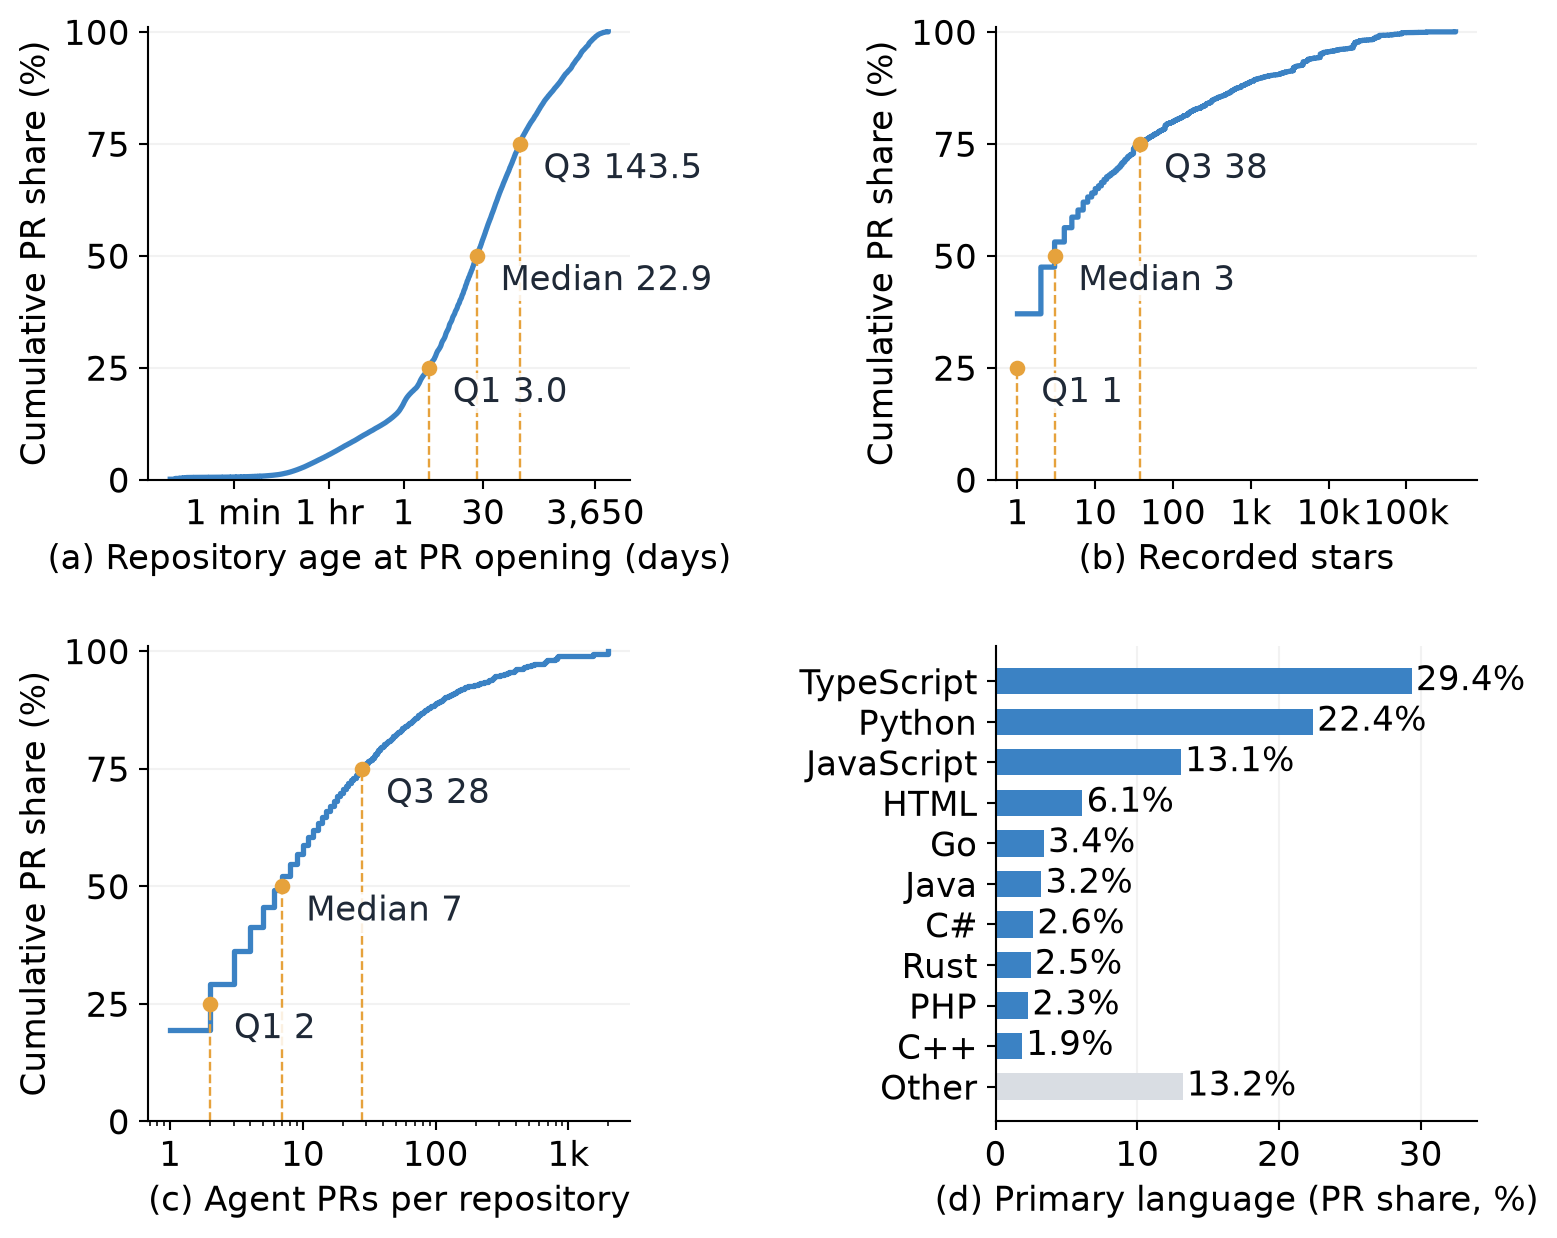
\includegraphics[width=\columnwidth]{figures/repository-background-reference-style-13pt.png}
\caption{Repository context of agent-authored PRs. Percentages are calculated over PRs with available values for each attribute. Panels (a)--(c) show cumulative PR shares on logarithmic x-axes. Panel (d) shows the ten most common primary languages, with the remaining 234 grouped as Other.}
\label{fig:repository_background}
\end{figure}

\subsection{PR Timeline Construction}
\label{sec:method_timeline}

Feedback refers to recorded \texttt{Comment} or \texttt{Review} events posted by an account other than the PR author, with timestamps strictly later than the PR opening time. These events are grouped as feedback because PR comments and reviews can guide subsequent changes by coding agents~\cite{liAIDevStudyingAICodingAgents2026,github2025copilotReviewExperience}.

For each PR, the timeline combines \texttt{Open}, \texttt{Comment}, \texttt{Review}, and \texttt{Commit} records linked to that PR. Each record identifies the account, event type, and timestamp. The earliest \texttt{Open} record identifies the PR opening time and author account. Records are ordered by timestamp, with code commits recorded separately from feedback.

The first feedback event is the earliest event that meets the definition above. Comments and reviews posted by the PR author do not qualify, but the author's later code commits remain in the timeline. When a \texttt{Comment} and a \texttt{Review} have the same timestamp, the \texttt{Comment} is selected using a fixed tie-breaking rule. Measures of who provides the first feedback include only PRs with feedback.

\subsection{Baseline construction}
\label{sec:baseline_construction}

Human- and bot-authored PRs serve as references for feedback and integration in agentic contributions. Both groups were collected through the same GitHub GraphQL API procedure, including PR records and their associated events. They are distinguished using the author signals described in Section~\ref{sec:data_collection_structure}. Each PR is linked to its events by repository and PR number, with GraphQL PR identifiers mapped to this pair where available. The available human and bot baseline records span PR creation dates from 2025-06-01 to 2025-11-14. Within this period, duplicate records with the same repository and PR number are reduced to one record per PR, keeping the earliest recorded creation time. Table~\ref{tab:analysis_data_and_users} reports the resulting groups.

These comparisons describe how feedback and integration patterns vary across agent-, human-, and bot-authored PRs. Across all three author groups, PR records are linked to events by repository and PR number and deduplicated by retaining the record with the earliest creation timestamp. The baselines provide context for the observed differences.

\subsection{Human-Agent PR Workflow Model}
\label{sec:method_workflow_model}

Recent research examines discussions among developers triggered by automated review comments~\cite{schaefDeveloperAnalyzerInteractions2024}. This motivates examining both who participates in the discussion and what feedback they provide, captured here as participation and feedback. Research on human and LLM review comments further distinguishes comment types from whether developers resolve them~\cite{goldmanWhatTypesCode2025}. This distinction motivates examining revision separately from feedback, focusing on the code changes that follow it. Finally, research on pull-based development examines merge decisions and processing time~\cite{gousiosExploratoryPullBased2014}. Integration connects the preceding interactions to the PR's observed status. These perspectives motivate four research questions that characterize RQ1 Participation, RQ2 Feedback, RQ3 Revision, and RQ4 Integration within the same PR timeline (Figure~\ref{fig:method_rq_workflow_timeline}).

RQ1 examines which PRs receive feedback and who provides the first feedback. For PRs with feedback, RQ2 examines its channels, forms, and content. RQ3 then examines code changes after feedback, including their timing, authors, and size. RQ4 relates these interaction patterns to whether PRs are merged, closed without merging, or still open at data collection.

\begin{figure*}[t]
    \centering
    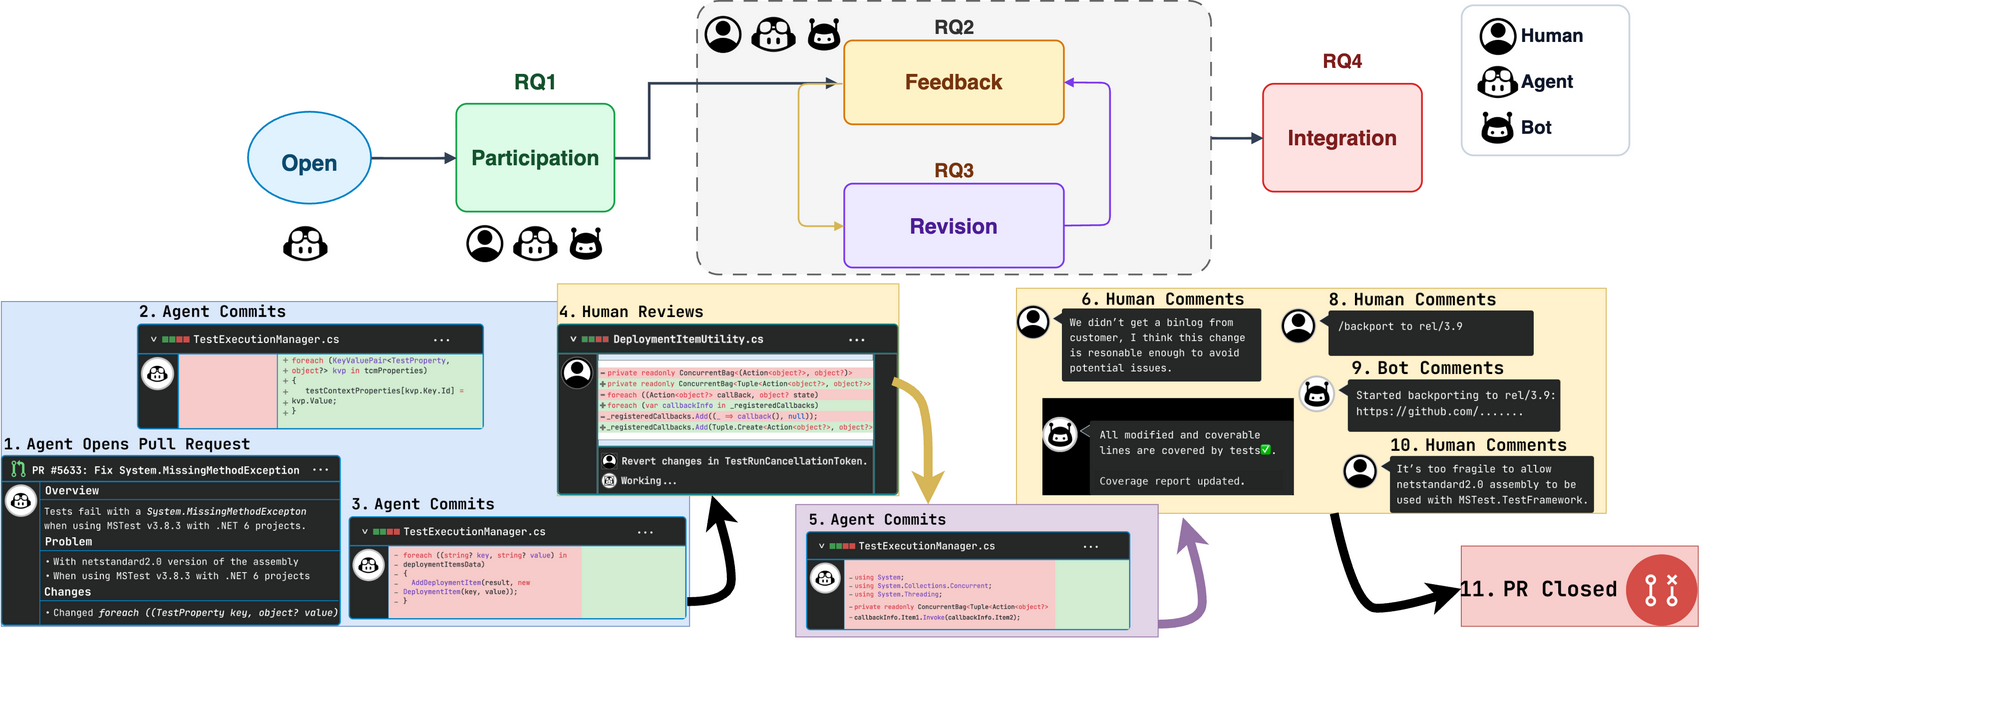
\includegraphics[width=\textwidth]{figures/fig_method_rq_workflow_timeline.png}
    \caption{Overview of the four research questions and an example PR timeline. The upper panel shows the research questions of participation, feedback, revision, and integration at their relative positions in a PR timeline, where feedback and revision may repeat. The lower panel illustrates feedback, revision, and closure in PR \href{https://github.com/microsoft/testfx/pull/5633}{microsoft/testfx\#5633}.}
    \label{fig:method_rq_workflow_timeline}
\end{figure*}

\subsection{Taxonomy Construction}
\label{sec:method_taxonomy_construction}

\subsubsection{RQ1: Participation}
\label{sec:method_rq1_entry}

\runinhead{Feedback and Participants}
RQ1 examines how many PRs receive feedback and who provides the first feedback.
The share of PRs receiving feedback is calculated before and after removing empty messages and specified status or boilerplate messages, such as deployment notices and CI summaries.
Section~\ref{sec:method_validation} details these filtering rules.
Both calculations use all PRs in each author group as the denominator and count a PR if it has at least one feedback event.
After filtering, the earliest remaining feedback event identifies the first feedback provider for each PR.

The first feedback provider is classified as Human, Agent, or Automation bot using the signals in Section~\ref{sec:data_collection_structure}.
The automated rules left 15 accounts unclassified.
Manual inspection assigned these accounts to Human (10), Agent (1), and Automation bot (4).
Only the first feedback event remaining after applying the message-filtering rules in Section~\ref{sec:method_validation} is used, so each PR contributes to only one category.
Category shares use all PRs with at least one remaining feedback event within each author group as the denominator.

\runinhead{Human Participant Profiles}
For agent-authored PRs whose first feedback after message filtering comes from a human, the provider is matched to the public user profiles introduced in Section~\ref{sec:data_collection_structure}.
Matching uses GitHub usernames converted to lowercase with surrounding whitespace removed.
Matched profiles provide account-creation dates and public contribution counts for the account measures defined below.
PRs without the required profile data remain in the feedback analysis but are excluded from comparisons based on these measures.

\runinhead{Public GitHub Footprint Score}
The public GitHub footprint score combines account age and public contribution counts.
For each user $u$, $\mathrm{tenure}(u)$ is the number of days from account creation to the latest user-profile collection timestamp.
Public contribution volume is defined as
$\mathrm{contrib}(u)=\#\mathrm{commits}(u)+\#\mathrm{PRs}(u)+\#\mathrm{reviews}(u)+\#\mathrm{issues}(u)$,
using the one-year window recorded in the user-profile dataset.
Both components are transformed using $\log(1+x)$ and capped at their 5th and 95th percentiles.
The transformed components are then min--max normalized to $[0,1]$ across all eligible user profiles.
The resulting values, $\widehat{\mathrm{tenure}}(u)$ and $\widehat{\mathrm{contrib}}(u)$, receive equal weights:
\[
\mathrm{footprint}(u)
=0.5\,\widehat{\mathrm{tenure}}(u)
+0.5\,\widehat{\mathrm{contrib}}(u).
\]

\runinhead{Footprint Groups}
Score quartiles are calculated among human participants in agent-authored PRs with available scores.
The 25th, 50th, and 75th percentiles define four groups, Q1 to Q4, from the lowest to the highest scores.
For PRs whose first feedback comes from a human with an available score, the PRs are grouped by that person's score quartile.
Figure~\ref{fig:rq1_human_footprint} shows the score distribution and the share of these PRs in each group.

\begin{figure}[tbp]
  \centering
  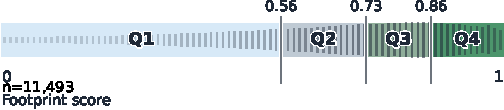
\includegraphics[width=\columnwidth]{figures/fig_rq1_footprint_score_strip.pdf}
  \vspace{0.12em}
  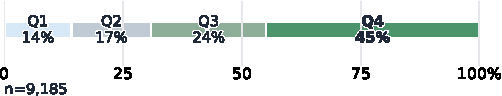
\includegraphics[width=\columnwidth]{figures/fig_rq1_human_triager_quartiles.pdf}
  \caption{Top: human participants' footprint scores and quartile boundaries.
Bottom: PR shares by the first feedback provider's quartile, restricted to PRs whose first feedback after filtering comes from a human with an available score.}
  \Description{Two vertically stacked plots.
  The score-distribution plot is a quartile strip of equal-weight account footprint scores from zero to one with density marks and quartile cut points near 0.56, 0.73, and 0.86.
  The first-retained-human-triager plot is a single stacked percentage bar for scoreable first retained human triagers, ordered from Q1 on the left to Q4 on the right.}
  \label{fig:rq1_human_footprint}
\end{figure}

\subsubsection{RQ2: Feedback}
\label{sec:method_rq2_feedback}

RQ2 examines feedback events on agent-authored PRs after applying the message filters in Section~\ref{sec:method_validation}.
Each feedback event is analyzed separately, so a PR can be associated with multiple feedback events.
The recorded feedback type distinguishes two channels, Comment and Review.
Within each channel, feedback is further grouped by provider type.

\runinhead{Feedback actors}
Feedback providers are classified as Human, Agent, or Automation bot using the account classification described in Section~\ref{sec:method_rq1_entry}.
The share of each provider type is calculated across all feedback events after filtering and separately for comments and reviews.
For the separate calculations, the denominator is the number of comments or reviews, respectively.

Human feedback providers are matched to the public user profiles and assigned to the footprint quartiles defined in Section~\ref{sec:method_rq1_entry}.
Feedback from human accounts without an available footprint score remains in the analysis and is reported separately.

\runinhead{Text Features}
Prior work has examined textual features of review comments~\cite{rahmanPredictingUsefulnessCode2017} and identified verbosity and information presentation as concerns in bot communication~\cite{wesselDontDisturbMe2021}.
Motivated by these studies, the analysis focuses on feedback length and format.
Length is measured by word and line counts for messages with available, nonempty text.
Format is characterized using text-matching rules for code-block markers, tables, lists, summary-like structures, and status-related expressions.
Their frequencies and the distributions of feedback length are summarized by provider type, separately for comments and reviews.

\runinhead{Intent Taxonomy}
To describe what the feedback concerns, RQ2 groups messages by their primary intent.
Prior research has used comment categories to compare human-written and LLM-generated code reviews~\cite{goldmanWhatTypesCode2025}.
Motivated by this work, the taxonomy distinguishes seven categories: \textit{Functional}, \textit{Maintainability}, \textit{Documentation}, \textit{Discussion}, \textit{Process}, \textit{Validation}, and \textit{Non-actionable}.
Each feedback event receives one primary label.

\textit{Functional} concerns incorrect or missing behavior.
\textit{Maintainability} concerns code clarity and structure.
\textit{Documentation} covers requests to change documentation or explanatory text.
\textit{Process} covers build, CI, deployment, and integration requests.
\textit{Validation} covers requests for tests, reproduction steps, or other evidence.
\textit{Discussion} covers questions and clarification without a specific change request.
\textit{Non-actionable} covers approvals, acknowledgments, and other messages without a request for further action or clarification.
Generated feedback is classified by its content using the same categories.
For messages containing multiple requests, the primary label represents the dominant request.

\runinhead{Intent Labeling}
Human annotation supports the development and assessment of the LLM classifier.
Prior work has also assessed LLM-based review classification using a manually labeled sample of 100 comments~\cite{goldmanWhatTypesCode2025}.
In this study, sampling covers different PR author types, feedback providers, merge states, and feedback and revision patterns.
Up to four events were selected from each stratum, producing 187 candidates.
Selection within strata favored shorter messages with explicit requests and excluded status-only messages.
A stratified allocation of approximately 70\% of these candidates, with rounding within strata, yielded 141 events for human annotation.

Two annotators independently assigned primary intent labels to the 141 events.
They then discussed disagreements and revised labels for 41 events.
After this discussion, their labels agreed on 104 events, with Cohen's $\kappa=0.683$.
The remaining 37 events were unresolved and excluded from the reference set used for classifier development and evaluation.
Following the existing split, the reference set contained 75 development events and 29 evaluation events.

The development set supplied examples for the classification prompt.
Model and prompt configurations were compared on the 29-event evaluation subset.
The selected configuration uses \texttt{gpt-4o-mini}, two examples per category, and batches of 20 feedback events.
None of the evaluation events appears among the prompt examples.
The model returns one primary intent label for each event.
On the evaluation subset, this configuration matched the human reference labels for 20 of 29 events, yielding 0.690 accuracy and 0.676 weighted-F1.
Weighted-F1 averages category-level F1 scores according to their frequencies in this subset.
All outputs contained a valid category label.
The selected configuration was then applied to the remaining feedback events.

\subsubsection{RQ3: Revision}
\label{sec:method_rq3_cycles}

RQ3 examines whether code commits follow feedback and how these changes unfold within a PR.
The analysis uses the PR timelines defined in Section~\ref{sec:method_timeline} to group feedback events and subsequent commits into cycles.
These cycles are constructed before applying the message-content filters used in RQ2.

\runinhead{Blocks and cycles}
Consecutive feedback events with no intervening commit form a \emph{feedback block}.
The commits that follow this block, before the next feedback event, form its \emph{response block}.
A feedback block and a response block containing at least one commit form one \emph{feedback-response cycle}.
Multiple commits within the same response block count as one cycle.
A feedback block with no subsequent commit does not form a cycle.

Only commits recorded after PR opening and before any recorded merge or closure are included.
Commits whose messages match predefined merge, squash, or rebase patterns are also excluded to avoid counting these operations as revisions following feedback.
The remaining commits and feedback events are ordered by timestamp.
At identical timestamps, comments precede reviews, and both precede commits.
Events with the same timestamp and type are ordered by their identifiers to ensure a consistent ordering.
A commit with the same timestamp as the preceding feedback might hence form a cycle with zero waiting time.

\runinhead{PR pathways}
Prior work describes code review as an iterative process in which reviewer comments are followed by revisions~\cite{sadowskiModernCodeReview2018}.
To characterize how this process unfolds in PR timelines, the pathway classification distinguishes whether feedback occurs and whether it is followed by one or multiple revision cycles.
Cycle counts alone do not show whether further feedback appears after the last revision.
The classification therefore also distinguishes PRs whose final feedback block follows the last included commit.
These distinctions define five pathways, with each PR assigned to exactly one using the rules below.

\textit{No visible feedback}. The PR contains no feedback events.
\textit{Feedback without code response}. Feedback is present, but no cycle is formed and the PR does not meet the late-feedback rule below.
\textit{Single-feedback response cycle}. The PR contains exactly one cycle and does not meet the late-feedback rule.
\textit{Multi-feedback response cycle}. The PR contains two or more cycles and does not meet the late-feedback rule.
\textit{Late feedback after final code change}. The final feedback block follows the last included commit, with no subsequent commit.

The late-feedback rule takes precedence over cycle count.
PRs in this category may contain zero, one, or multiple earlier cycles.

\runinhead{Cycle timing}
Cycle latency is the elapsed time from the last feedback event in a feedback block to the first commit in its response block.
Each cycle contributes one observation, so a PR with multiple cycles contributes multiple observations.
Feedback blocks without a subsequent commit are excluded from latency summaries.
The distribution is summarized using the median, interquartile range, and upper percentiles.
A separate summary includes only cycles whose feedback blocks contain at least one event retained by the message filters in Section~\ref{sec:method_validation}.
This subset uses the original cycle boundaries and latency values.

\runinhead{Revision size}
Prior work measures PR size using commit counts, changed lines, and changed files~\cite{gousiosExploratoryPullBased2014}.
In this study, these measures can also describe revisions within each cycle and across each PR.
For each cycle, commits are counted and changed lines and file counts are summed across its response block.
Changed lines are calculated as additions plus deletions when both values are available.
File counts come from the per-commit \texttt{changed\_files} field, so a file modified in multiple commits is counted more than once.

For each cycle, total changed lines are also divided by the number of feedback events to describe change volume relative to feedback volume.
For each PR, included commits are divided into those before and after its first feedback event.
PRs without feedback or subsequent commits remain in the summaries with zero commits and changes after feedback.

\runinhead{Revision accounts}
For each response block, GitHub accounts are extracted from the author fields of its commits.
The committer field is used when no author account is available.

\subsubsection{RQ4: Integration}
\label{sec:method_taxonomy_rq4}

RQ4 examines how the PR pathways defined in Section~\ref{sec:method_rq3_cycles} relate to observed PR states.
These states are determined from the PR metadata in the dataset snapshot used for analysis, using GitHub's merge and close timestamps.\footnote{GitHub GraphQL API, \texttt{PullRequest.mergedAt} and \texttt{PullRequest.closedAt}: \url{https://docs.github.com/en/graphql/reference/pulls\#pullrequest}.}
A PR is classified as \emph{merged} if a GitHub merge timestamp is present, including when a close timestamp is also recorded.
Otherwise, a recorded close timestamp identifies a PR as \emph{closed without merge}.
PRs with neither timestamp are classified as \emph{open}, consistent with their recorded state.

The pathway comparison includes all agent-authored PRs in the study sample, selected by creation time regardless of their observed state.
PRs without visible feedback are included in the corresponding pathway defined in Section~\ref{sec:method_rq3_cycles}.
Within each pathway, the proportions of merged, closed-without-merge, and open PRs use all PRs in that pathway as the denominator.
Merge-rate differences are reported in percentage points by subtracting the merge rate of the no-visible-feedback pathway from that of each other pathway.

Additional comparisons group agent-authored PRs by the provider, primary intent, or text form of their first feedback event remaining after message filtering.
Each comparison includes PRs with the corresponding information available.
The footprint comparison further restricts the sample to PRs whose first retained feedback comes from a human with an available score, using the quartiles defined in Section~\ref{sec:method_rq1_entry}.
For each comparison, the reference proportion is calculated across its eligible PRs before grouping.
Differences in merge and open proportions are reported in percentage points relative to this reference.

Time from first feedback to merge or closure is calculated separately from the PR timelines used in RQ3.
For each measure, the first feedback timestamp is subtracted from the corresponding GitHub timestamp, and the duration is expressed in days.
Only PRs whose first feedback strictly precedes that timestamp contribute to the timing summary.
Time to closure includes merged PRs with a recorded close timestamp.

For merged PRs in the late-feedback pathway, the last feedback timestamp is compared with the merge timestamp to determine whether feedback occurs before, at the same recorded time as, or after merging.
PRs in the late-feedback pathway are also grouped by whether their final feedback block contains comments, reviews, or both.
For blocks containing reviews, merge proportions are further summarized by the review states recorded by GitHub, including blocks in which all reviews indicate approval.\footnote{GitHub records approval as \texttt{APPROVED} in \texttt{PullRequestReview.state}: \url{https://docs.github.com/en/graphql/reference/pulls\#pullrequestreviewstate}.}

\subsection{Validation and Robustness}
\label{sec:method_validation}

\runinhead{Retained-feedback sensitivity}
We evaluate four feedback boundaries.
\emph{Raw visible feedback} includes all post-open non-author PR comments and reviews.
\emph{Relaxed retained feedback} removes only empty-body events and comments or reviews from known status, deployment, CI, helper, routing, release, security-scan, and administrative service accounts.
% ORIGINAL:
% \emph{Main retained feedback}, used in RQ1--RQ4, further excludes deployment previews, CI/check/build summaries, helper invitations, routing or assignment commands, generated summary shells without review findings, release/version notices, CLA/administrative messages, security-scan notices, and other boilerplate/status-only events matched by the retained-feedback codebook.
\emph{Main retained feedback} further excludes deployment previews, CI/check/build summaries, helper invitations, routing or assignment commands, generated summary shells without review findings, release/version notices, CLA/administrative messages, security-scan notices, and other boilerplate/status-only events matched by the retained-feedback codebook.
We use this main retained boundary for retained-entry, feedback-actor, body-form, and intent summaries.
Structural pathway analyses keep the broader visible-feedback timeline and state the denominator where results appear.
The filter is content/status based, and agent or bot messages are retained if they contain substantive review, process, evidence, or change-request content.
To sanity-check, the authors jointly audited a stratified sample of 100 retained and 100 excluded feedback events and found no systematic rule violations.
\emph{Strict retained feedback} additionally removes short non-actionable acknowledgments and terminal signals, such as approval-only, thanks-only, LGTM-only, no-comments/no-issues, and merge-ready comments, unless they contain actionable cues such as fix, test, validate, refactor, or failure-related requests.
Across non-raw retained definitions, retained-feedback entry remains a minority of agent-authored PRs.
Relaxed, main, and strict retained boundaries cover 13.3\%, 10.5\%, and 10.3\% of agent-authored PRs, respectively.

\runinhead{Footprint-score sensitivity}
We recompute footprint strata using tenure-only, contribution-only, and alternative tenure/contribution weights, while keeping each PR's first-human-responder assignment fixed.
PRs whose first human responder lacks scoreable metadata remain outside these footprint-stratified summaries.

\runinhead{Endpoint censoring sensitivity}
Because open or without-close endpoints may reflect the collection boundary, we repeat integration summaries after excluding PRs opened near the end of the study window and after exclusions that leave one top agent out, so that endpoint patterns are not affected by late-window censoring or a single dominant agent.
Across the main and sensitivity summaries, proportions are reported with counts and denominators, with Wilson or difference intervals for selected actor, syntax, and endpoint contrasts in the artifact.

\runinhead{Repository characteristics}
To examine how workflow patterns vary across repositories, agent-authored PRs are grouped by repository ownership, repository age at PR creation, and the number of sampled PRs from each repository.
Within each group, the analysis calculates the proportions of PRs with visible feedback, at least one feedback-response cycle, and a recorded merge.

Ownership distinguishes repositories owned by personal accounts from those owned by organizations.
Repository age is divided into four descriptive groups: up to 90 days, over 90 to 365 days, over 365 to 1,095 days, and over 1,095 days.
The number of sampled agent-authored PRs per repository is grouped as 1, 2--10, 11--100, and more than 100.

To show variation across repositories, the three proportions are also calculated separately for each repository within each group.
Their distributions are displayed as empirical cumulative distribution functions.
A repository can appear in more than one age group because its PRs may have been created at different repository ages.

Group differences are estimated using linear probability models with group membership as the predictor.
The models use standard errors clustered by repository to account for dependence among PRs from the same repository~\cite{cameronClusterRobustInference2015}.
Differences are reported in percentage points with 95\% confidence intervals.

For each repository characteristic, an F-test assesses whether the groups have equal proportions for each of the three measures.
Holm correction is applied across the nine tests and separately across all group-to-reference comparisons~\cite{holmMultipleTestProcedure1979}.
Groups with unknown characteristics are excluded from these tests.

\section{Results}
\label{results}

\subsection{RQ1: Entry}
\label{sec:rq1_results}

\runinhead{Entry denominators}
% ORIGINAL:
% Among 325,523 agent-authored PRs, 86,504 (26.6\%) have raw entry through a non-author comment or review, 34,049 (10.5\%) retain review-relevant feedback after filtering, and 33,502 (10.3\%) contain at least one feedback-response cycle.
Among 325,523 agent-authored PRs, 86,504 (26.6\%) have raw entry through a non-author comment or review, 34,049 (10.5\%) retain review-relevant feedback after filtering, and 33,502 (10.3\%) contain at least one feedback-response cycle.
The retained-entry denominator is therefore much narrower than the raw visible PR-thread record, but it is the relevant denominator for asking who first enters the PR thread with substantive retained feedback.

\runinhead{First retained entry actor}
In the 34,049 retained-entry PRs, the first retained actor is nearly split between humans (17,037 PRs, 50.0\%, Wilson 95\% CI [49.5, 50.6]) and agents (16,132 PRs, 47.4\%, [46.8, 47.9]).
Automation bots account for 856 PRs (2.5\%, [2.4, 2.7]) and unresolved agent/bot accounts for 24 PRs (0.1\%, [0.0, 0.1]).
RQ1's answer is therefore that retained PR-thread feedback occurs for a minority of agent-authored PRs.
When it occurs, the first retained entry actor is almost evenly split between humans and agents.

\runinhead{First human triager footprint}
Figure~\ref{fig:rq1_human_footprint} stratifies the human side of RQ1 using an equal-weight account footprint score with 0.5 normalized account tenure and 0.5 normalized public contribution volume.
The score-distribution plot shows the covered account distribution over this continuous score, with quartile cut points at 0.56, 0.73, and 0.86.
Among the 17,037 PRs whose first retained entry came from a human, 9,185 (53.9\%) join to a scoreable engaging account in the footprint table.
The first-human-triager plot displays this scoreable subset.
Q1 accounts provide the first retained human entry for 1,301 PRs (14.2\%), Q2 accounts for 1,540 PRs (16.8\%), Q3 accounts for 2,219 PRs (24.2\%), and Q4 accounts for 4,125 PRs (44.9\%).
The remaining 7,852 first-human PRs (46.1\% of the full first-human denominator) come from accounts whose metadata is unavailable and are therefore not assigned to quartiles.
These no-metadata PRs correspond to 2,809 unique first-human triager accounts that appear in the retained-feedbacks but have no match in the user metadata and footprint-score table.
The no-metadata stratum denotes uncovered metadata.
Thus, among the 53.9\% of first-human retained-entry PRs with scoreable metadata, developers in the largest footprint quartile account for 44.9\% of first human entries.
\FloatBarrier

\subsection{RQ2: Feedback}
\label{sec:rq2_results}

\runinhead{Feedback channels and syntax features}
Figure~\ref{fig:rq2_feedback_body_syntax} summarizes the channel and body-shape side of RQ2.
The RQ2 denominator is 76,936 retained feedback events with deduplicated event IDs.
Most retained feedback appears as PR comments, with 56,589 events (73.6\%).
GitHub review events account for the remaining 20,347 events (26.4\%).
Figure~\ref{fig:rq2_feedback_body_syntax} shows that feedback on agent-authored PRs is mostly thread comment feedback rather than review events.

\begin{figure*}[tbp]
  \centering
  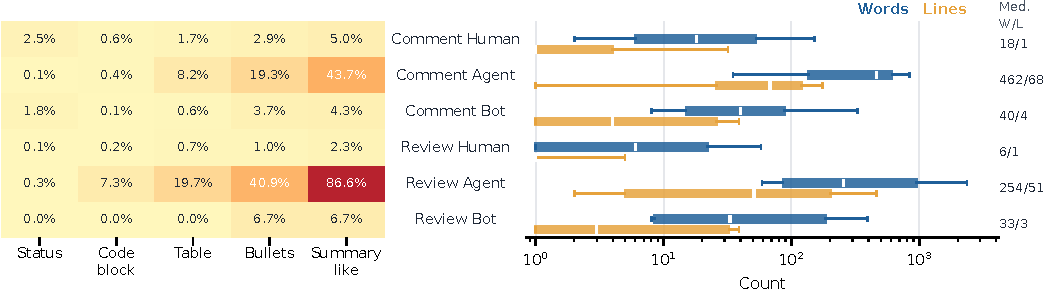
\includegraphics[width=\textwidth]{figures/fig_rq2_feedback_body_syntax.pdf}
  \caption{RQ2 feedback body form by channel and actor. Left heatmap cells report the percentage of retained feedback events in each channel-actor group whose body matches each syntax feature. Right boxplots summarize feedback-body word and line counts on a log scale. Boxes show the IQR, whiskers P10--P90, numeric labels mark medians. Outliers hidden. Bot=automation bot.}
  \Description{A two-panel figure with shared group labels in the middle.
  The left side is a heatmap for Comment Human, Comment Agent, Comment Bot, Review Human, Review Agent, and Review Bot across Status, Code block, Table, Bullets, and Summary-like syntax features.
  The strongest cells are summary-like Review Agent feedback at 86.6\%, summary-like Comment Agent feedback at 43.7\%, bullets in Review Agent feedback at 40.9\%, and bullets in Comment Agent feedback at 19.3\%.
  The right side is a horizontal interval plot of word and line counts.
  Human comments have a median of 18 words and 1 line.
  Agent comments have a median of 462 words and 68 lines.
  Human reviews have a median of 6 words and 1 line.
  Agent reviews have a median of 254 words and 51 lines.}
  \label{fig:rq2_feedback_body_syntax}
\end{figure*}

The body text also differs strongly by actor.
Human feedback is usually short.
Human comments have a median of 18 words and one line, while human reviews have a median of 6 words and one line.
The one-line pattern for human reviews is real in the data because the 75th percentile is still one line, and the 90th percentile is five lines.
Agent feedback is much longer.
Agent comments have a median of 462 words and 68 lines, while agent reviews have a median of 254 words and 51 lines.

The syntax features tell the same story in another way.
Human feedback rarely uses structured markup features such as code blocks, tables, bullets, or summary-like format.
Agent feedback uses these features much more often, notably in review events.
Compared with human reviews, agent reviews are +84.3 pp higher on summary-like form (95\% CI [+83.6, +85.0]) and +39.9 pp higher on bullets ([+39.0, +40.9]); in comments, the summary-like gap is +38.6 pp ([+38.0, +39.3]).
Figure~\ref{fig:rq2_feedback_body_syntax} also shows that comments are the larger feedback channel, and agent feedback is more structured.

\runinhead{Feedback actors}
The top row of Figure~\ref{fig:rq2_feedback_actor_intent} answers the actor part of RQ2 across all retained feedback and by channel.
On all retained feedback, agents provide 35,115 events (45.6\%).
Human accounts provide 40,231 events (52.3\%), and automation bots provide 1,590 (2.1\%).
This all-event view differs from RQ1 because it asks who enters first, while RQ2 asks who provides the feedback events that appear after entry.

\begin{figure}[tbp]
  \centering
  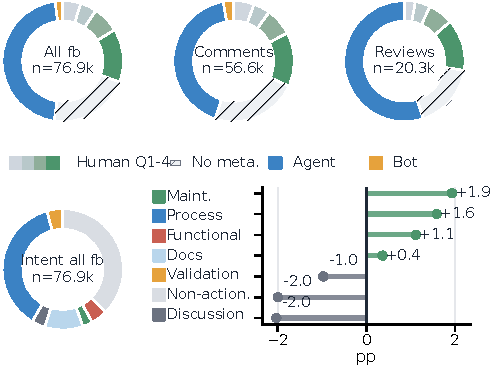
\includegraphics[width=\columnwidth]{figures/fig_rq2_feedback_actor_intent.pdf}
  % ORIGINAL: \caption{RQ2 event-level feedback actors and intent mix for 76,936 retained feedback events. Panels show actor shares, primary-intent shares, and review-minus-comment intent differences in pp. Maint.=Maintainability, Docs=Documentation, Non-action.=Non-actionable, Bot=automation bot.}
  \caption{RQ2 event-level feedback actors and intent mix for 76,936 retained feedback events. Panels show actor shares, primary-intent shares, and review-minus-comment intent differences in pp. Maint.=Maintainability, Docs=Documentation, Non-action.=Non-actionable, Bot=automation bot.}
  \Description{A compact multi-panel figure.
  The top row shows donut charts for all retained feedback, comments, and reviews.
  Across all retained feedback, Q1 humans are 5\%, Q2 humans are 4\%, Q3 humans are 7\%, Q4 humans are 14\%, no-metadata humans are 22\%, agents are 46\%, and automation bots are 2\%.
  In comments, agents are 42\%.
  In reviews, agents are 55\%.
  The lower-left panel is a donut chart for 76,936 labeled retained feedback events.
  Non-actionable feedback and Process feedback are each about 37\%, Documentation feedback is about 10\%, and the remaining slices are smaller.
  The lower-right panel is a diverging point-and-line chart of review-minus-comment percentage-point differences, sorted from largest positive difference to largest negative difference.
  % ORIGINAL: Every intent category appears in both comments and reviews.
  Every intent category appears in both comments and reviews.
  The largest channel differences are small, around two percentage points.}
  \label{fig:rq2_feedback_actor_intent}
\end{figure}

The actor mix changes by channel.
Agents provide 11,188 of 20,347 reviews (55.0\%) versus 23,927 of 56,589 comments (42.3\%), a +12.7 pp difference between reviews and comments (95\% CI [+11.9, +13.5]).
Automation bots provide 2.8\% of comments but only 0.1\% of reviews.
Figure~\ref{fig:rq2_feedback_actor_intent} shows review events are more agent-heavy than comments.

The human side is not evenly distributed across footprint strata.
Among humans, Q1 provides 3,682 retained feedback events (4.8\% of all retained feedback events), Q2 provides 3,362 events (4.4\%), Q3 provides 5,525 events (7.2\%), and Q4 provides 10,977 events (14.3\%).
Another 16,685 events (21.7\%) come from humans without footprint metadata.
As in RQ1, this no-metadata group denotes accounts that are not able to join the footprint-score table.
Within the human strata, Q4 accounts have the majority of human feedback.

% ORIGINAL: \runinhead{Feedback intent}
\runinhead{Feedback intent}
% ORIGINAL: The bottom row of Figure~\ref{fig:rq2_feedback_actor_intent} summarizes the intent labels attached to feedback events.
% ORIGINAL: The bottom row of Figure~\ref{fig:rq2_feedback_actor_intent} summarizes descriptive intent labels attached to feedback events.
The bottom row of Figure~\ref{fig:rq2_feedback_actor_intent} summarizes intent labels attached to feedback events.
% ORIGINAL: The overall distribution is concentrated in a few intent types.
The overall distribution is concentrated in a few intent types.
Non-actionable feedback accounts for 28,837 events (37.5\%).
Process feedback has 28,683 events (37.3\%).
Documentation feedback is the next largest group with 7,836 events (10.2\%).
% ORIGINAL: The remaining intent groups are smaller than 5\% of all feedback events.
The remaining intent groups are smaller than 5\% of all feedback events.

The comparison between reviews and comments is more stable than the actor and body-shape comparison.
% ORIGINAL: Every intent category appears in both comments and reviews, and their shares are similar.
Every intent category appears in both comments and reviews, and their shares are similar.
For reviews, non-actionable and process feedback account for 36.0\% and 38.4\%.
For comments, they account for 38.0\% and 36.9\%.
The largest absolute channel differences are about two percentage points (pp).
Discussion feedback is lower in reviews than in comments, Maintainability feedback is higher in reviews, and Process feedback is slightly higher in reviews.
These differences are much smaller than the actor and syntax differences shown above.

% simplify for page restriction
Figures~\ref{fig:rq2_feedback_body_syntax} and~\ref{fig:rq2_feedback_actor_intent} show that retained feedback differs most by channel, actor, and body form.
% ORIGINAL: Intent differences between comments and reviews are smaller.
Intent differences between comments and reviews are smaller.

\subsection{RQ3: Feedback-response Cycles}
\label{sec:rq3_results}

\runinhead{Workflow pathway composition}
Over all, most agent-authored PRs do not enter a feedback-response pathway.
There are 239,019 PRs (73.4\%) with no visible feedback.
Another 44,177 PRs (13.6\%) receive feedback but have no later response-eligible commit.
Explicit response cycles are less common.
Only 16,446 PRs (5.1\%) have one feedback-response cycle, and 4,682 PRs (1.4\%) have multiple cycles.
The remaining 21,199 PRs (6.5\%) end with late feedback after the final code change.
Thus, RQ3 shows that response cycles are uncommon.
Most PRs have no visible feedback or feedback without later code response.

\runinhead{Cycle latency}
Among agent-authored PRs with feedback-response cycles, the latency table contains 59,159 cycles across 33,502 PRs.
The median cycle latency is 7.0 minutes.
Only 54 of 59,159 cycles (0.09\%) have zero latency from same-timestamp ordering, so the 7.0-minute median is not driven by the tie-breaking rule.
The majority of cycles are fast, with 62.1\% occurring within 10 minutes and 88.9\% occurring within 60 minutes.
The distribution is however long-tailed, with P90 at 76.1 minutes and P95 at 483.2 minutes.
The retained-feedback cycle subset is similar at the median.
It contains 31,394 retained cycles across 16,775 PRs with a median latency of 7.1 minutes and P90 of 65.0 minutes.
Because cycle latency is skewed, we emphasize medians and upper percentiles rather than averages.
Figure~\ref{fig:results_actor_intent_cycle_latency} visualizes the skew with compact log-scale interval strips.
% simplify for page restriction
% ORIGINAL: Figure~\ref{fig:results_actor_intent_cycle_latency} shows the same median-fast, tail-heavy pattern by actor and intent.
Figure~\ref{fig:results_actor_intent_cycle_latency} shows the same median-fast, tail-heavy pattern by actor and intent.

\begin{figure}[tbp]
  \centering
  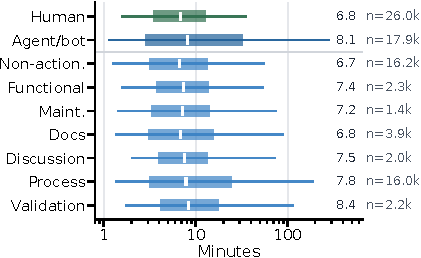
\includegraphics[width=0.9\columnwidth]{figures/fig_results_actor_intent_cycle_latency.pdf}
  \caption{Cycle-level feedback-response latency for 59,159 visible feedback-response cycles across 33,502 agent-authored PRs. Actor rows stratify cycles by feedback actor. Agent/bot combines agent accounts and automation bots. Intent rows pool cycles across actors and stratify by primary feedback intent. Thick bands show IQR, whiskers P10--P90, white ticks/numbers medians, and right labels row counts.}
  \Description{Compact horizontal interval-strip figure.
  The first two rows compare cycle latency for human feedback and Agent/bot feedback.
  % ORIGINAL: The remaining rows pool feedback cycles across actors and compare cycle latency by primary feedback intent.
  The remaining rows pool feedback cycles across actors and compare cycle latency by primary feedback intent.
  Most medians are in the single-digit-minute range, while P90 endpoints extend much farther on the log scale.}
  \label{fig:results_actor_intent_cycle_latency}
\end{figure}

\runinhead{Response}
In the 59,159 agent-authored feedback-response cycles, response commit accounts are often not limited to the PR author.
The largest response-actor category is PR author + others, covering 25,825 cycles (43.7\%).
Mixed non-author response accounts cover another 19,848 cycles (33.6\%).
Non-author human-only response blocks account for 7,955 cycles (13.4\%), while PR-author-only response blocks account for 4,290 cycles (7.3\%).
Non-author agent/bot-only response blocks are rather rare at 1,241 cycles (2.1\%).
The five strata are mutually exclusive.
They are PR-author-only, PR author plus other accounts, non-author human-only, non-author agent/bot-only, and mixed non-author accounts with both human and agent/bot non-author commit accounts.
These categories report commit accounts attached to GitHub commits.

Figure~\ref{fig:results_post_feedback_revision} reports the code-response magnitude after visible feedback.
For PRs with raw visible feedback, changed lines remain sparse (median 0; P90 631; P95 2,074), but the feedback-with-code-response subset is larger at the median and tail (median 120; P90 3,024; P95 8,164).
The cycle-count strata show that repeated cycles are associated with larger response.
One-cycle PRs have a median of 72 post-feedback changed lines, whereas PRs with six or more cycles have one of 1,414 changed lines.
The upper tail also grows with cycle count, from P95 of 6,010 changed lines for one-cycle PRs to P95 of 49,791 changed lines for PRs with six or more cycles.
The outlier check reports changed-lines P95 of 8,164 in the visible-feedback and code-response denominator, 6,440 after dropping the top 1\%, and 3,407 after dropping PRs above 10,000 changed lines.
% simplify for page restriction
There is hence a two-level pattern.
Many raw-visible-feedback PRs have no measured post-feedback code response, while cycle-bearing PRs have larger, heavy-tailed responses.

\begin{figure}[tbp]
  \centering
  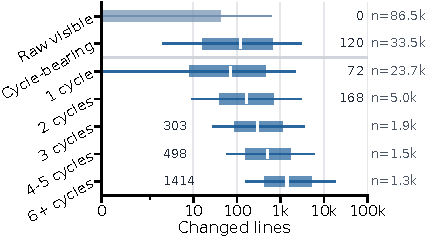
\includegraphics[width=0.9\columnwidth]{figures/fig_results_post_feedback_revision.pdf}
  \caption{Code-response magnitude after visible feedback. Bands show IQR, whiskers P10--P90, white ticks/numbers mark medians. Outliers are hidden.}
  \Description{Interval-strip figure showing post-feedback changed lines.
  The first rows compare the raw-visible-feedback and cycle-bearing denominators.
  The remaining rows show that changed lines increase as the number of visible feedback-response cycles grows.}
  \label{fig:results_post_feedback_revision}
\end{figure}

\subsection{RQ4: Integration}
\label{sec:rq4_results}

\runinhead{Merge outcomes over the entry-cycle composition}
Figure~\ref{fig:results_integration_by_pathway} composes the RQ1 entry and RQ3 feedback-response pathway summaries with integration endpoints.
The unit of analysis is the agent-authored PR, and each is assigned one endpoint category.
The endpoint categories are merged, closed without merging, and open PR.
The pathway-specific endpoint percentages use the same PR-level denominators introduced in RQ3.
These denominators are 239,019 no-visible-feedback PRs, 44,177 feedback-without-code-response PRs, 16,446 single-cycle PRs, 4,682 multi-cycle PRs, and 21,199 late-feedback PRs.
No-visible-feedback PRs are the pathway reference, with a 68.3\% merge rate.
Relative to that reference, feedback-without-code-response PRs are nearly unchanged (+0.1 pp, 95\% CI [-0.3, +0.6]), single-cycle PRs are lower (-5.5 pp, [-6.3, -4.7]), multi-cycle PRs are similar (+1.1 pp, [-0.2, +2.5]), and late-feedback PRs are higher (+12.3 pp, [+11.7, +12.9]); single-cycle PRs also have the largest open PR share (20.7\%).

\begin{figure}[tbp]
  \centering
  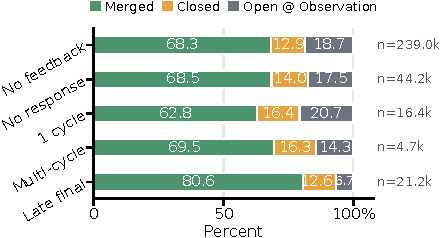
\includegraphics[width=0.9\columnwidth]{figures/fig_results_integration_by_pathway.pdf}
  \caption{PR-level RQ4 integration endpoint composition by feedback-response pathway for 325,523 agent-authored PRs. Each PR is assigned one endpoint (merged, closed without merge, or open PR at observation). Each row sums to 100\%, and right labels report pathway denominators.}
  \Description{Stacked horizontal bar chart of integration endpoint percentages by feedback-response pathway.
  No-visible-feedback and feedback-without-code-response PRs merge at about 68\%, single-cycle PRs merge at 62.8\%, multi-cycle PRs merge at 69.5\%, and late-feedback PRs merge at 80.6\%.}
  \label{fig:results_integration_by_pathway}
\end{figure}

\runinhead{Terminal feedback as an integration signal}
% ORIGINAL:
% Figure~\ref{fig:results_rq4_endpoint_delta} summarizes selected actor, intent, and first-human footprint-quartile merged-rate contrasts.
% ORIGINAL: Figure~\ref{fig:results_rq4_endpoint_delta} summarizes selected actor, descriptive intent-stratum, and first-human footprint-quartile merged-rate contrasts.
% ORIGINAL: The late-feedback pathway requires a terminal-workflow interpretation.
% ORIGINAL: By definition, this pathway means that the final feedback block starts after the final code change and has no later response block.
The late-feedback pathway needs a terminal interpretation because its final feedback block starts after the final code change and has no later response block.
% ORIGINAL: The terminal diagnostic breakdown supports this interpretation: 11,940 late-feedback PRs end with a review-only final feedback block, and these PRs merge at 89.0\%.
% ORIGINAL: The same breakdown also shows that 8,282 late-feedback PRs end with an \texttt{APPROVED}-only review state, and these PRs merge at 93.8\%.
The terminal diagnostic breakdown supports this interpretation: 11,940 late-feedback PRs end with a review-only final feedback block and merge at 89.0\%; another 8,282 end with an \texttt{APPROVED}-only review state and merge at 93.8\%.
% ORIGINAL: Among merged late-feedback PRs, 3,536 have their last feedback recorded after the merge timestamp and 9,371 have their last feedback within five minutes before merge.
% ORIGINAL: This pattern indicates that late feedback often records approval-like or merge-adjacent integration evidence.
% ORIGINAL: Among merged late-feedback PRs, 3,536 record last feedback after merge and 9,371 within five minutes before merge, suggesting approval-like or merge-adjacent integration evidence.
Among merged late-feedback PRs, 3,536 record last feedback after the merge timestamp and 9,371 within five minutes before merge.
This pattern indicates that late feedback often records approval-like or merge-adjacent integration evidence.
% ORIGINAL: The body-form endpoint breakdown is also consistent with that interpretation: summary-like first retained bodies are 10.7 pp above the body-form baseline on merged, while short and long plain-text bodies are 4.2 and 3.6 pp below it, respectively.
% ORIGINAL: For open PR endpoints, the same breakdown shows summary-like first retained bodies 4.8 pp below the body-form baseline, while short and long plain-text bodies are 2.0 and 1.6 pp above it, respectively.
% ORIGINAL: The body-form endpoint breakdown points the same way: summary-like first bodies are +10.7 pp from the merged baseline and -4.8 pp from the open-PR baseline, while short and long plain text are -4.2/-3.6 pp on merged and +2.0/+1.6 pp on open PRs.
The body-form endpoint breakdown is consistent with that interpretation: summary-like first retained bodies are 10.7 pp above the body-form baseline on merged, while short and long plain-text bodies are 4.2 and 3.6 pp below it.
For open PR endpoints, the pattern reverses: summary-like first retained bodies are 4.8 pp below the body-form baseline, while short and long plain-text bodies are 2.0 and 1.6 pp above it.
% ORIGINAL: Figure~\ref{fig:results_rq4_endpoint_delta} summarizes selected actor, intent stratum, and first-human footprint-quartile merged-rate contrasts.

\begin{figure}[tbp]
  \centering
  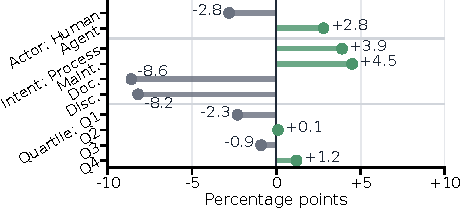
\includegraphics[width=0.9\columnwidth]{figures/fig_results_rq4_endpoint_delta.pdf}
  \caption{PR-level RQ4 selected merged-rate differences from construct-specific baselines. Zero is the merged rate within each construct's covered subset before stratification (first retained actor, first retained intent/body form, or scoreable first-human triagers). Points are pp differences from that baseline.}
  \Description{Three compact diverging point-and-line plots of merged-rate differences.
  The actor panel contrasts human and agent first-retained entry, the intent panel contrasts selected feedback intents, and the quartile panel contrasts scoreable first-human-triager footprint strata.}
  \label{fig:results_rq4_endpoint_delta}
\end{figure}

\runinhead{Integrated interpretation}
% ORIGINAL:
% Figure~\ref{fig:results_rq4_endpoint_delta} summarizes selected RQ1 and RQ2 actor, intent, and first-human footprint-quartile strata as merged-rate differences from construct-specific endpoint baselines.
% ORIGINAL: Figure~\ref{fig:results_rq4_endpoint_delta} summarizes selected RQ1 and RQ2 actor, descriptive intent, and first-human footprint-quartile strata as merged-rate differences from construct-specific endpoint baselines.
% ORIGINAL: Figure~\ref{fig:results_rq4_endpoint_delta} summarizes selected RQ1 and RQ2 actor, intent, and first-human footprint-quartile strata as merged-rate differences from construct-specific endpoint baselines.
Figure~\ref{fig:results_rq4_endpoint_delta} reports merged-rate differences from construct-specific baselines for selected actor, intent, and first-human footprint-quartile strata.
For first retained actor, the agent row is 2.8 pp above the actor baseline on merged, while the human row is 2.8 pp below it.
% ORIGINAL:
% For first retained intent, Process and Maintainability rows are 3.9 and 4.5 pp above the intent baseline on merged, while Documentation and Discussion are 8.6 and 8.2 pp below it.
% ORIGINAL: For first retained descriptive intent, Process and Maintainability rows are 3.9 and 4.5 pp above the intent baseline on merged, while Documentation and Discussion are 8.6 and 8.2 pp below it.
For the first retained intent, Process and Maintainability rows are 3.9 and 4.5 pp above the intent baseline on merged, while Documentation and Discussion are 8.6 and 8.2 pp below it.
For scoreable first-human triagers, Q1 and Q3 are 2.3 and 0.9 pp below the footprint baseline on merged, while Q2 and Q4 are 0.1 and 1.2 pp above it.
% ORIGINAL:
% Documentation-first PRs are 13.4 pp above the intent baseline on open PR, and Q1 first-human triagers are 7.0 pp above the footprint baseline.
% ORIGINAL: Documentation-first PRs are 13.4 pp above the descriptive-intent baseline on open PR, and Q1 first-human triagers are 7.0 pp above the footprint baseline.
% ORIGINAL: For open PR endpoints, the endpoint breakdown behind Figure~\ref{fig:results_rq4_endpoint_delta} shows the largest positive contrasts for documentation-first PRs (+13.4 pp from the intent baseline) and Q1 first-human triagers (+7.0 pp from the footprint baseline).
% ORIGINAL: For open PR endpoints, the breakdown behind Figure~\ref{fig:results_rq4_endpoint_delta} has the largest positive contrasts for documentation-first PRs (+13.4 pp) and Q1 first-human triagers (+7.0 pp).
For open PR endpoints, the breakdown behind Figure~\ref{fig:results_rq4_endpoint_delta} shows the largest positive contrasts in documentation-first PRs and Q1 first-human triagers: +13.4 pp from the intent baseline and +7.0 pp from the footprint baseline, respectively.
% ORIGINAL: Summary-like first retained bodies are 4.8 pp below the body-form baseline on open PR, and Q4 first-human triagers are 3.9 pp below the footprint baseline.
% ORIGINAL: Summary-like first bodies and Q4 first-human triagers are lower on open PRs (-4.8 and -3.9 pp).
Summary-like first retained bodies are 4.8 pp below the body-form baseline on open PR, and Q4 first-human triagers are 3.9 pp below the footprint baseline.
The Q1 row has the smallest quartile denominator (1,301 PRs).
% simplify for page restriction
Together, Figures~\ref{fig:results_integration_by_pathway} and~\ref{fig:results_rq4_endpoint_delta} show that integration endpoints vary with the preceding workflow pathway, so similar merge labels can hide different entry, feedback, and response-cycle states.

\FloatBarrier

\section{Discussion}
\label{discussion}

% REJECTED COMPRESSION:
% Agent-authored PRs should be read as engagement workflows, not only as accepted or rejected changes.
% For ADLC work on evaluation, observability, and guardrails~\cite{bergmannAgentDevelopmentLifecycle2026,googleNewSDLCVibeCoding2026}, this adds the repository boundary: after a PR opens, observability should cover whether review-relevant feedback appears, who provides it, whether code response follows, and whether the final feedback is terminal.
% For workflow measurement, a merge label should be paired with the preceding pathway, because no-feedback, feedback-without-code-response, single-cycle, multi-cycle, and late-feedback PRs represent different review and verification states.
We study agent-authored PRs as engagement workflows, not as acceptance outcomes.
The results do not collapse to one signal.
Retained feedback, response cycles, revision, and integration capture different parts of the PR path.
A raw "reviewed" or "merged" label can therefore mix PRs with no retained feedback, feedback without response, iterative cycles, terminal approval-like feedback, or larger revisions.

\subsection{Implications for the Agent Development Lifecycle (ADLC)}

Existing ADLC discussions give names to evaluation, observability, and guardrails around agents~\cite{bergmannAgentDevelopmentLifecycle2026,googleNewSDLCVibeCoding2026}.
Our data add the repository boundary.
An agent patch has not finished its lifecycle when a PR opens.
It still has to engage with, or fail to engage with public feedback, actor participation, code response, and integration.
Only 26.6\% of agent-authored PRs receive raw visible feedback, retained review-relevant feedback remains 10.3\% to 13.3\% across filtering boundaries, and retained-feedback first entry is nearly split between humans and agents.
For ADLC, observability should cover repository uptake as well as agent-internal execution: which generated changes receive review-relevant feedback, who provides it, and whether later PR activity produces code response.

\subsection{Workflow Metrics for Agent-authored Software Changes}

The pathway results explain why merge should not stand alone.
A merged agent-authored PR may have no visible feedback, feedback without code response, one response cycle, repeated cycles, or terminal merge-adjacent feedback.
These states point to different review and verification states, but they now collapse under one endpoint label.
Integration should therefore be read together with the preceding pathway to see whether feedback appeared, whether a code response followed, and whether the final feedback block was terminal.

\subsection{Threats to Validity and Future Work}
\label{sec:threats_validity}

% REJECTED COMPRESSION:
% The corpus prioritizes precision and repository-visible signals.
% Following prior agent-authored PR mining work~\cite{popescu2026autonomous, watanabeUseAgenticCoding2026, watanabeHowAICoding2026}, we identify agent-authored PRs from public account, branch, and text signals, which cannot recover private, disabled, or human-account-mediated agent use.
% The author groups are not repository-matched controls, so cross-group and endpoint contrasts are descriptive workflow associations rather than causal author-type or reviewer effects.
% The workflow reconstruction captures comments, reviews, commits, endpoints, and timestamps, but not private review, local agent iteration, IDE/chat traces, or agent-runtime state.
% Retained feedback is a conservative review-relevant subset, footprint strata summarize public trace profiles rather than expertise, and intent labels are aggregate descriptive signals.
% Endpoint rates for all visible-feedback pathways are unchanged under the 30-day mature-PR filter, and late-feedback merge rates remain 79.1--81.1\% after leaving out each top agent family in turn.
% Future work can connect these workflows to downstream maintenance signals and richer IDE, chat, CI, and agent-runtime traces.
% PAGE-FIT ORIGINAL:
% The corpus prioritizes precision and repository-visible signals.
% Following prior agent-authored PR mining work~\cite{popescu2026autonomous, watanabeUseAgenticCoding2026, watanabeHowAICoding2026}, we identify agent-authored PRs from public account, branch, and text signals.
% This improves attribution precision, but it cannot recover agent-assisted work whose signals are private, disabled, or recorded under human accounts.
% The same issue can affect the human baseline, and the author groups are not repository-matched controls.
% We therefore treat cross-group and endpoint contrasts as descriptive workflow associations rather than causal author-type or reviewer effects.
%
% The workflow reconstruction captures the public PR thread rather than the full development process.
% It includes comments, reviews, commits, endpoints, and timestamps, but not private review, local agent iteration, IDE/chat traces, or agent-runtime state.
% Feedback-response cycles and post-feedback revision are temporal signals.
% Code activity followed feedback, but fuller traces would be needed to establish causality.
% Body-form and terminal-review endpoint patterns may also reflect repository automation and review conventions.
%
% The retained-feedback filter and public GitHub footprint score introduce construct limits.
% Retained feedback is a conservative review-relevant subset, not a complete measure of all useful feedback.
% Footprint strata summarize public trace profiles, not actual expertise or quality.
% No-metadata accounts remain uncovered, and footprint-stratified results generalize only to scoreable human triagers.
% Endpoint robustness checks reduce sensitivity to two design choices.
% Endpoint rates for all visible-feedback pathways are unchanged under the 30-day mature-PR filter, and late-feedback merge rates remain 79.1--81.1\% after leaving out each top agent family in turn.
% We therefore keep null-hypothesis significance testing out of the main claims, while keeping interval and effect-size outputs for audit in the artifact.
% The findings are most directly informative for public GitHub repositories during the 2025--2026 study window where agent activity is visibly marked and PR-based development is routine.
% Future work can connect these workflow patterns to downstream maintenance signals such as defects, reverts, and long-term ownership, and combine PR traces with IDE, chat, CI, and agent-runtime data.
The corpus prioritizes precision and repository-visible signals.
Following prior agent-authored PR mining work~\cite{popescu2026autonomous, watanabeUseAgenticCoding2026, watanabeHowAICoding2026}, the study identifies agent-authored PRs from public account, branch, and text signals.
This improves attribution precision, but it cannot recover agent-assisted work hidden by private settings, disabled signals, or human accounts.
% PAGE-FIT ORIGINAL: The human baseline may have the same issue, and the author groups are not repository-matched controls; cross-group and endpoint contrasts are therefore descriptive workflow associations, not causal author-type or reviewer effects.
The same issue may affect the human baseline, and non-repository-matched author groups make cross-group and endpoint contrasts descriptive rather than causal.

The workflow reconstruction captures public PR-thread traces: comments, reviews, commits, endpoints, and timestamps.
It omits private review, local agent iteration, IDE/chat traces, and agent-runtime state.
Feedback-response cycles and post-feedback revision are temporal signals; fuller traces would be needed to establish causality.
Body-form and terminal-review endpoint patterns may also reflect repository automation and review conventions.

The retained-feedback filter and public GitHub footprint score also limit the constructs.
Retained feedback is a conservative review-relevant subset, not a complete measure of all useful feedback.
Footprint strata summarize public trace profiles rather than expertise or quality, and no-metadata accounts remain uncovered.
% PAGE-FIT ORIGINAL: Endpoint robustness checks reduce sensitivity to two design choices: endpoint rates for all visible-feedback pathways are unchanged under the 30-day mature-PR filter, and late-feedback merge rates remain 79.1--81.1\% after leaving out each top agent family in turn.
Two endpoint robustness checks are stable: pathway endpoint rates are unchanged under the 30-day mature-PR filter, and late-feedback merge rates remain 79.1--81.1\% in top-agent leave-one-out checks.
% PAGE-FIT ORIGINAL: Null-hypothesis significance testing is therefore kept out of the main claims, while interval and effect-size outputs remain in the artifact.
Null-hypothesis significance testing is kept out of the main claims, while interval and effect-size outputs remain in the artifact.
% PAGE-FIT ORIGINAL: The findings are most directly informative for public GitHub repositories during the 2025--2026 study window where agent activity is visibly marked and PR-based development is routine.
% PAGE-FIT ORIGINAL: Future work can connect these workflow patterns to downstream maintenance signals such as defects, reverts, and long-term ownership, and combine PR traces with IDE, chat, CI, and agent-runtime data.
The findings are most directly informative for public GitHub repositories during 2025--2026 where agent activity is visibly marked and PR-based development is routine.
Future work can connect these workflows to downstream maintenance signals and richer IDE, chat, CI, and agent-runtime traces.

\section{Related Work}
\label{sec:related_work}

% REJECTED COMPRESSION:
% Coding-agent work has moved from completion and chat toward tools that plan tasks, edit files, run checks, and interact with repository infrastructure~\cite{pengImpactAIDeveloper2023,chenCodeMeMe2025,treudeHowDevelopersInteract2025}, while benchmark studies still emphasize task completion and synthetic issue resolution~\cite{wangSurveyLargeLanguage2024,liangSWEBenchIllusionWhen2025a}.
% PR and review research treats pull requests as socio-technical workflows shaped by contributor, project, review, and mining-trace factors~\cite{tsayInfluenceSocialTechnical2014,kononenkoStudyingPullRequest2018,yuWaitItDeterminants2015,deyEffectTechnicalSocial2020,kalliamvakouPromisesPerilsMining2014}.
% Review-automation and human-agent feedback studies show that automation changes review dynamics and that human reviewers can provide broader feedback than agents~\cite{wesselEffectsAdoptingCode2020,wesselQualityGatekeepersInvestigating2022,wesselDontDisturbMe2021,zhongHumanAISynergyAgentic2026}.
% Recent studies of agent-authored PRs examine acceptance, merge outcomes, activity patterns, code changes, PR descriptions, tests, security, failed PRs, references, human responses, actionable loops, and minimal-feedback merges~\cite{liAIDevStudyingAICodingAgents2026,liRiseAITeammates2025a,watanabeUseAgenticCoding2026,popescu2026autonomous,yoshiokaLetsMakeEvery2026,ogenrwotHowAICoding2026,haqueAutonomousAgentsContribute2026,siddiqSecurityAgeAI2026,ehsaniWhereAICodingAgentsFail2026,khemissiHumansIntegrateAgentsFix2026,watanabeHowAICoding2026,nachumaWhenAITeammates2026,gaoAutopilotEmpiricalStudy2026}.
% We complement this cluster by reconstructing raw and retained feedback entry, first-entry actor, feedback actor and intent, response-cycle latency, post-feedback revision, and pathway-conditioned integration endpoints.
\paragraph{Coding Agents in Software Development}
% PAGE-FIT ORIGINAL:
% AI support for programming has moved from local completion and chat assistance toward tools that can plan tasks, edit multiple files, run checks, and interact with repository infrastructure~\cite{pengImpactAIDeveloper2023,chenCodeMeMe2025,treudeHowDevelopersInteract2025}.
% At the same time, benchmark-oriented studies still emphasize task completion, benchmark accuracy, or synthetic issue resolution~\cite{wangSurveyLargeLanguage2024,liangSWEBenchIllusionWhen2025a}.
% These studies are useful for measuring coding capability, but they say less about what happens after an agent-produced change becomes a repository artifact.
% Recent work also shows that human feedback remains important during agent-assisted planning and code generation~\cite{takerngsaksiriHumanIntheLoopSoftwareDevelopment2025b}.
% Our study focuses on the later repository-facing stage after an agent-authored PR is opened.
AI support for programming has moved from local completion and chat asssitance toward tools that can plan tasks, edit multiple files, run checks, and interact with repository infrastructure~\cite{pengImpactAIDeveloper2023,chenCodeMeMe2025,treudeHowDevelopersInteract2025}.
Benchmark studies still emphasize task completion, benchmark accuracy, or issue resolution~\cite{wangSurveyLargeLanguage2024,liangSWEBenchIllusionWhen2025a}.
% PAGE-FIT ORIGINAL: These studies measure coding capability more than what happens after an agent-produced change becomes a repository artifact.
% PAGE-FIT ORIGINAL: Recent work also shows that human feedback remains important during agent-assisted planning and code generation~\cite{takerngsaksiriHumanIntheLoopSoftwareDevelopment2025b}.
These studies measure coding capability more than repository uptake after an agent-produced change becomes a PR, while recent work shows that human feedback remains important during agent-assisted planning and code generation~\cite{takerngsaksiriHumanIntheLoopSoftwareDevelopment2025b}.
This study examines the later repository-facing stage after PR creation.

\paragraph{Pull Requests as Socio-Technical Workflows}
% PAGE-FIT ORIGINAL:
% Pull requests are not only containers for code changes.
% They are socio-technical workflows shaped by technical risk, contributor reputation, project norms, and reviewer workload~\cite{tsayInfluenceSocialTechnical2014,kononenkoStudyingPullRequest2018}.
% Prior work shows that PR latency is associated with contributor familiarity, project load, and PR characteristics~\cite{yuWaitItDeterminants2015}, and that review and acceptance outcomes depend on both technical and social factors rather than code features alone~\cite{deyEffectTechnicalSocial2020}.
% Recent work also studies PRs as broader coordination structures, including interventions that accelerate overdue PRs and views of how PRs and issues organize development~\cite{maddilaNudgeAcceleratingOverdue2023,desouzaRevealingSoftwareDevelopment2024}.
% Mining studies have also warned that large-scale GitHub analyses inherit missing actions, noisy account labels, and selection bias from public repository traces~\cite{kalliamvakouPromisesPerilsMining2014}.
% This literature motivates our use of public PR actions as reproducible workflow traces while also motivating the construct limits discussed in Section~\ref{sec:threats_validity}.
Pull requests are socio-technical workflows, not only containers for code changes, and are shaped by technical risk, contributor reputation, project norms, and reviewer workload~\cite{tsayInfluenceSocialTechnical2014,kononenkoStudyingPullRequest2018}.
Prior work links PR latency to contributor familiarity, project load, and PR characteristics~\cite{yuWaitItDeterminants2015}, and shows that review and acceptance outcomes depend on technical and social factors rather than code features alone~\cite{deyEffectTechnicalSocial2020}.
% PAGE-FIT ORIGINAL: Recent work also studies PRs as broader coordination structures, including interventions for overdue PRs and views of how PRs and issues organize development~\cite{maddilaNudgeAcceleratingOverdue2023,desouzaRevealingSoftwareDevelopment2024}.
Recent work also studies PRs as coordination structures, including overdue-PR interventions and links between PRs and issues~\cite{maddilaNudgeAcceleratingOverdue2023,desouzaRevealingSoftwareDevelopment2024}.
% PAGE-FIT ORIGINAL: Mining studies warn that large-scale GitHub analyses inherit missing actions, noisy account labels, and selection bias from public repository traces~\cite{kalliamvakouPromisesPerilsMining2014}.
% PAGE-FIT ORIGINAL: This literature motivates the use of public PR actions as reproducible workflow traces and the construct limits discussed in Section~\ref{sec:threats_validity}.
Mining studies warn that large-scale GitHub analyses inherit missing actions, noisy account labels, and selection bias~\cite{kalliamvakouPromisesPerilsMining2014}; this motivates the construct limits in Section~\ref{sec:threats_validity}.

\paragraph{Review Automation and Human-Agent Feedback}
% PAGE-FIT ORIGINAL:
% Modern PR threads contain human review, automation-bot messages, and increasingly agent-mediated review.
% Code-review bot research shows that automation can alter pull-request dynamics, developer workflows, and notification burden~\cite{wesselEffectsAdoptingCode2020,wesselQualityGatekeepersInvestigating2022,wesselDontDisturbMe2021}.
% Large-scale evidence from review conversations shows that human reviewers provide broader feedback than agents, including understanding, testing, and knowledge transfer~\cite{zhongHumanAISynergyAgentic2026}.
% It also reports more review iterations when humans review AI-generated code and lower adoption rates for AI suggestions than for human suggestions.
% This work motivates our actor layer, which separates humans, agents, and automation bots before analyzing response cycles, revision, and integration.
Modern PR threads contain human review, automation-bot messages, and increasingly agent-mediated review.
Code-review bot research shows that automation can alter pull-request dynamics, developer workflows, and notification burden~\cite{wesselEffectsAdoptingCode2020,wesselQualityGatekeepersInvestigating2022,wesselDontDisturbMe2021}.
Large-scale evidence from review conversations shows that human reviewers provide broader feedback than agents, including understanding, testing, and knowledge transfer, and that adoption differs for AI and human suggestions~\cite{zhongHumanAISynergyAgentic2026}.
This work motivates the actor layer, which separates humans, agents, and automation bots before analyzing response cycles, revision, and integration.

\paragraph{Empirical Studies of Agent-Authored Pull Requests}
% PAGE-FIT ORIGINAL:
% Recent empirical studies have made agent-authored PRs a rapidly growing target~\cite{liAIDevStudyingAICodingAgents2026,liRiseAITeammates2025a}.
% Some studies characterize acceptance, merge outcomes, activity patterns, code change over time, and broad attributes~\cite{watanabeUseAgenticCoding2026,popescu2026autonomous,yoshiokaLetsMakeEvery2026}.
% Others focus on specific quality and contribution metrics, including code modifications and PR-description consistency~\cite{ogenrwotHowAICoding2026}, test inclusion~\cite{haqueAutonomousAgentsContribute2026}, security-related PRs~\cite{siddiqSecurityAgeAI2026}, failed or rejected PRs~\cite{ehsaniWhereAICodingAgentsFail2026}, and cross-PR references in practice~\cite{khemissiHumansIntegrateAgentsFix2026}.
%
% The closest work examines review and collaboration signals around agent-authored PRs, including PR-description characteristics, human review responses, reviewer engagement, actionable review loops, and minimal-feedback merges~\cite{watanabeHowAICoding2026,nachumaWhenAITeammates2026,gaoAutopilotEmpiricalStudy2026}.
% Our paper complements this cluster by reconstructing the PR-thread workflow after PR creation.
% We analyze raw and retained feedback entry, first-entry actor, feedback actor and intent, response-cycle latency, post-feedback revision, and pathway-conditioned integration endpoints.
Recent empirical studies have made agent-authored PRs a rapidly growing target~\cite{liAIDevStudyingAICodingAgents2026,liRiseAITeammates2025a}.
Some characterize acceptance, merge outcomes, activity patterns, code change over time, and broad attributes~\cite{watanabeUseAgenticCoding2026,popescu2026autonomous,yoshiokaLetsMakeEvery2026}.
Others focus on code modifications and PR-description consistency~\cite{ogenrwotHowAICoding2026}, test inclusion~\cite{haqueAutonomousAgentsContribute2026}, security-related PRs~\cite{siddiqSecurityAgeAI2026}, failed or rejected PRs~\cite{ehsaniWhereAICodingAgentsFail2026}, and cross-PR references~\cite{khemissiHumansIntegrateAgentsFix2026}.

% PAGE-FIT ORIGINAL: The closest work examines review and collaboration signals around agent-authored PRs, including PR-description characteristics, human review responses, reviewer engagement, actionable review loops, and minimal-feedback merges~\cite{watanabeHowAICoding2026,nachumaWhenAITeammates2026,gaoAutopilotEmpiricalStudy2026}.
The closest work examines review and collaboration signals around agent-authored PRs, including PR descriptions, human responses, reviewer engagement, actionable loops, and minimal-feedback merges~\cite{watanabeHowAICoding2026,nachumaWhenAITeammates2026,gaoAutopilotEmpiricalStudy2026}.
% PAGE-FIT ORIGINAL: This paper complements that cluster by reconstructing the PR-thread workflow after PR creation: raw and retained feedback entry, first-entry actor, feedback actor and intent, response-cycle latency, post-feedback revision, and pathway-conditioned integration endpoints.
This paper complements that cluster by reconstructing raw and retained feedback entry, first-entry actor, feedback actor, and intent, response-cycle latency, post-feedback revision, and pathway-conditioned integration endpoints.

\section{Conclusions}
\label{conclusion}

We reframe agent-authored PRs as engagement workflows rather than binary outcomes. Only 26.6\% of 325,523 agent-authored PRs receive any visible feedback, and just 10.5\% carry feedback substantive enough to retain under our main filter. Where retained feedback appears, triage is nearly split between humans and agents, meaning close to half of the first-line review of agent work is itself performed by agents, a finding that merge rate alone cannot surface.
The pathway decomposition shows why this matters. No-feedback and feedback-without-response PRs together account for 87.0\% of the corpus, yet the remaining pathways diverge sharply. A ``merge'' label conflates PRs that were rubber-stamped, silently integrated, or genuinely revised, states that matter for trust and oversight but are invisible at the endpoint. By making entry, retained feedback, response cycles, and integration separately measurable, our framework offers the ADLC community a way to ask not just whether agent contributions are merged but also how.
% PAGE-FIT ORIGINAL:
% In this study, we examine agent-authored PRs as PR-thread engagement workflows, not as outcomes to be accepted or rejected.
% Our results show that retained feedback, feedback-response structure, post-feedback revision, and integration endpoints are distinct workflow signals that cannot be replaced by a single review or merge label.
% By distinguishing no-visible-feedback, feedback-without-code-response, single-cycle, multi-cycle, and late-feedback pathways, we provide a more precise basis for studying how coding agents enter real repository workflows.
% REJECTED PAGE-FIT CONCLUSION:
% Agent-authored PRs should be evaluated as repository-visible engagement workflows rather than binary outcomes.
% In 325,523 agent-authored PRs, only 26.6\% receive visible feedback and 10.5\% retain review-relevant feedback; when retained feedback appears, first triage is nearly split between humans and agents.
% Because no-feedback and feedback-without-response PRs account for 87.0\% of the corpus, merge labels conflate silent integration, approval-like closure, and genuinely revised PRs; entry, retained feedback, response cycles, revision, and integration should therefore be reported separately.

% ORIGINAL: 
\newpage
\bibliographystyle{IEEEtran}
\bibliography{phd_ziyou_sync_shared}

\end{document}
